%\documentclass[aps,preprintnumbers,showkeys,prd,twocolumn,groupedaddress,superscriptaddress]{revtex4-2}
\documentclass[10pt,prd,aps,showpacs,twocolumn,unsortedaddress]{revtex4-1}

%\documentclass[aps,preprintnumbers,draft,showkeys,prd,twocolumn,groupedaddress,superscriptaddress]{revtex4-2}
%%=======================================================================================
%% FRANK'S ADDITIONS
%%=======================================================================================
%% Make pages, sections and links clickable
\usepackage{hyperref} \hypersetup{ colorlinks=true, linkcolor=blue }
%% Allow for options on figure/includegraphics size, etc
\usepackage{graphicx}
%% Show line numbers
\usepackage{lineno}
%% For chemical elements like 4He, etc.
\usepackage[version=4]{mhchem} 
%% Bold and arrows for vector
%\usepackage{esvect}
%\usepackage{bm}
%% Use captions and subcaptions for figures and subfigures
\usepackage[caption=false]{subfig}
%\usepackage[font=footnotesize,labelfont={bf},tableposition=top]{caption}
%\usepackage[font=scriptsize,labelfont={bf}]{subcaption}
% Using multi rows in table
\usepackage{multirow}
\newcommand\he{{\ce{^{4}He}}}
\newcommand\pio{{\pi^0}}
\newcommand\pim{{\pi^-}}
\newcommand\dvmp{{\text{DV}\pio\text{P}}}
\renewcommand{\deg}{\ensuremath{^\circ}} 
%% Bracing/Parentheses
\newcommand\lr[1]{\left( #1\right) }
\newcommand\lrb[1]{\left[ #1\right] }
\newcommand\lrB[1]{\left\{ #1\right\} }
\newcommand\lra[1]{\left< #1\right> }
\newcommand\brac[2]{\left<#1 ~\big|~#2\right>}		
\newcommand\abv[1]{\left|#1 \right|}
%% Formatting and highlighting
\renewcommand\b[1]{{\textbf{#1}}}
\renewcommand\u[1]{{\underline{#1}}}
%% Referencing
\newcommand\Fig[1]{\b{{\u{{Fig. #1}}}}}
\newcommand\Figs[1]{\b{\u{Figs. #1}}}
\newcommand\Eq [1]{\b{\u{Eq. #1}}}
\newcommand\Eqs[1]{\b{\u{Eqs. #1}}}
\newcommand\Tab[1]{\b{\u{Table #1}}}
\newcommand\Part[1]{\b{\u{Part #1}}}
%\newcommand\Part[1]{\b{\u{Chapter #1}}}
\newcommand\Sec[1]{\b{\u{Section #1}}}
\newcommand\App[1]{\b{\u{Appendix #1}}}
\newcommand\delline{\vspace{-\baselineskip}}
\newcommand\moller{{M{\o}ller} }
\newcommand\elastic{e ~\he \rightarrow e ~\he  }
\newcommand\coherent{e ~\he \rightarrow e ~\he ~\pio }
\newcommand\decay{\pio \rightarrow \gamma ~\gamma }

%% ****** Start of file apstemplate.tex ****** %
%%
%%
%%   This file is part of the APS files in the REVTeX 4.2 distribution.
%%   Version 4.2a of REVTeX, January, 2015
%%
%%
%%   Copyright (c) 2015 The American Physical Society.
%%
%%   See the REVTeX 4 README file for restrictions and more information.
%%
%
% This is a template for producing manuscripts for use with REVTEX 4.2
% Copy this file to another name and then work on that file.
% That way, you always have this original template file to use.
%
% Group addresses by affiliation; use superscriptaddress for long
% author lists, or if there are many overlapping affiliations.
% For Phys. Rev. appearance, change preprint to twocolumn.
% Choose pra, prb, prc, prd, pre, prl, prstab, prstper, or rmp for journal
%  Add 'draft' option to mark overfull boxes with black boxes
%  Add 'showkeys' option to make keywords appear
%\documentclass[aps,prl,preprint,superscriptaddress]{revtex4-2}
%\documentclass[aps,prl,reprint,groupedaddress]{revtex4-2}

% You should use BibTeX and apsrev.bst for references
% Choosing a journal automatically selects the correct APS
% BibTeX style file (bst file), so only uncomment the line
% below if necessary.
%\bibliographystyle{apsrev4-2}

  \captionsetup[subfigure]{labelformat=brace}
\begin{document}

% Use the \preprint command to place your local institutional report
% number in the upper righthand corner of the title page in preprint mode.
% Multiple \preprint commands are allowed.
% Use the 'preprintnumbers' class option to override journal defaults
% to display numbers if necessary
\linenumbers
\preprint{Version 1 as of March 15th 2019 UConn}

%Title of paper
\title{Coherent Deeply Virtual $\pio$ Production off $\he$}
% repeat the \author .. \affiliation  etc. as needed
% \email, \thanks, \homepage, \altaffiliation all apply to the current
% author. Explanatory text should go in the []'s, actual e-mail
% address or url should go in the {}'s for \email and \homepage.
% Please use the appropriate macro foreach each type of information

% \affiliation command applies to all authors since the last
% \affiliation command. The \affiliation command should follow the
% other information
% \affiliation can be followed by \email, \homepage, \thanks as well.
\author{Frank Thanh Cao}
\email[]{franktcao@gmail.com}
%\homepage[]{Your web page}
%\thanks{you}
%\altaffiliation{}

\author{Kyungseon Joo}
\email[]{kjoo@phys.uconn.edu}
\affiliation{University of Connecticut}
\collaboration{CLAS Collaboration}

\author{Kawtar Hafidi}
\email[]{kjoo@jsifjsphys.uconn.edu}

\author{Mohammad Hattawy}
\email[]{kjoo@jsifjsphys.uconn.edu}

\author{Whitney Armstrong}
\email[]{kjoo@jsifjsphys.uconn.edu}
\affiliation{Argonne National Lab}
%\noaffiliation

%Collaboration name if desired (requires use of superscriptaddress
%option in \documentclass). \noaffiliation is required (may also be
%used with the \author command).
%\collaboration can be followed by \email, \homepage, \thanks as well.

\date{\today}

\begin{abstract}
This is the abstract.
\end{abstract}

% insert suggested keywords - APS authors don't need to do this
\keywords{Nuclear, DVMP, Pion, Neutral, helium, helium-4}

%\maketitle must follow title, authors, abstract, and keywords
\maketitle

% body of paper here - Use proper section commands
% References should be done using the \cite, \ref, and \label commands

%%%%%%%%%%%%%%%%%%%%%%%%%%%%%%%%%%%%%%%%%%%%%%%%%%%%%%%%%%%%%%%%%%%%%%%%%%%%%%%%%%%%%%%%%%%%%%%%%%%%
\section{Introduction \label{intro}}
\label{sect1}
%%%%%%%%%%%%%%%%%%%%%%%%%%%%%%%%%%%%%%%%%%%%%%%%%%%%%%%%%%%%%%%%%%%%%%%%%%%%%%%%%%%%%%%%%%%%%%%%%%%%
Content.
% Put \label in argument of \section for cross-referencing
%%%%%%%%%%%%%%%%%%%%%%%%%%%%%%%%%%%%%%%%%%%%%%%%%%%%%%%%%%%%%%%%%%%%%%%%%%%%%%%%%%%%%%%%%%%%%%%%%%%%
\section{Formalism \label{formalism}}
%%%%%%%%%%%%%%%%%%%%%%%%%%%%%%%%%%%%%%%%%%%%%%%%%%%%%%%%%%%%%%%%%%%%%%%%%%%%%%%%%%%%%%%%%%%%%%%%%%%%

%%%%%%%%%%%%%%%%%%%%%%%%%%%%%%%%%%%%%%%%%%%%%%%%%%
\subsection{Measuring Beam Spin Asymmetry 
\label{measure_bsa}}
%%%%%%%%%%%%%%%%%%%%%%%%%%%%%%%%%%%%%%%%%%%%%%%%%%
\begin{figure}[h!]
    \captionsetup{width=0.48\linewidth, format = hang}
    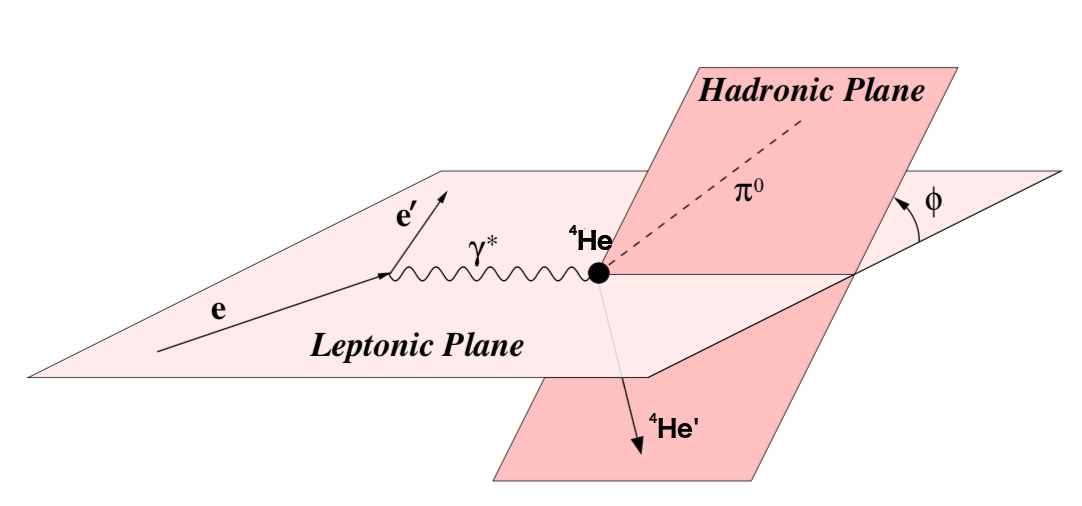
\includegraphics[width = 0.48\textwidth]{figs/theory/hadronic_phi_nuclear}
    \caption[]{Schematic of coherent $\dvmp$ reaction }
    \label{schematic}
\end{figure}
A schematic of coherent $\pio$ electroproduction off the $\he$ (coherent $\dvmp$) can be seen in \Fig{\ref{schematic}}, 
where the incoming electron $e$ emits a virtual photon $\gamma^*$ and is scattered $e'$ off the target helium $\he$. 
The incoming and outgoing electron form the scattering or leptonic plane, while the recoiling $\he$ and $\pio$ form the reaction or hadronic plane. 
The direction of the outgoing $\pio$ then determines the angle $\phi$ between the leptonic and hadronic planes. 

The virtual photon is described by the value of the four-momentum transfer $Q^2$, energy transfer $\nu$, and polarization $\epsilon$:
\begin{align}
\nu      &= E - E' \\
Q^2      &= 4 E E' \sin^2\lr{\theta_{e'/2}} \\
\epsilon &= \lrb{ 1 + 2\frac{\nu^2}{Q^2}\tan^2\lr{\theta_{e'}/2}}^{-1}
\end{align}

where $E, E'$ are the initial and final energies of the electron, respectively, and $\theta_{e'}$ is the scattered electron's polar angle in the lab frame.


%%%%%%%%%%%%%%%%%%%%%%%%%%%%%%%%%%%%%%%%%%%%%%%%%%
\subsection{Ji's Formulation  
\label{bsa}}
%%%%%%%%%%%%%%%%%%%%%%%%%%%%%%%%%%%%%%%%%%%%%%%%%%
\begin{figure}[h!]
    \captionsetup{width=0.48\linewidth, format = hang}
    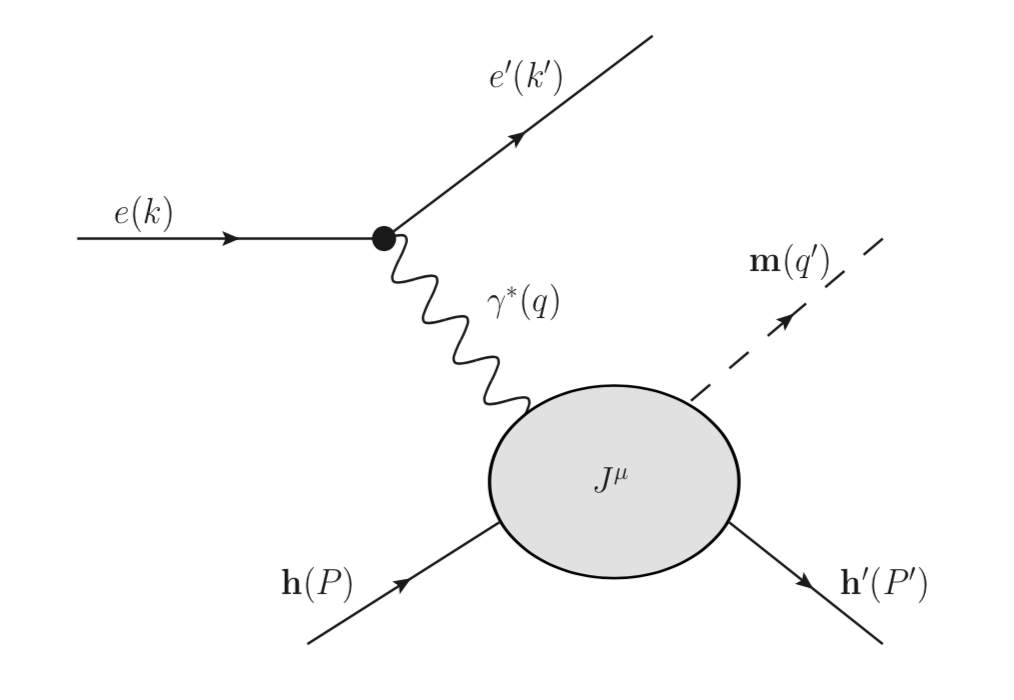
\includegraphics[width = 0.48\textwidth]{figs/theory/dvmp}
    \caption[]{Schematic of coherent $\dvmp$ reaction }
    \label{dvmp}
\end{figure}
  Most generally, the electroproduction differential cross section can be written as
  %\begin{widetext}
  \begin{align}
    \begin{split}
    d\sigma &= \frac{d^5\sigma}{dydxdtd\phi_{k'}d\phi_{q'}} 
    \\
    &= \lrb{\frac1{\lr{2\pi}^5}\frac{xy}{32Q^2\sqrt{1+\lr{\frac{2Mx}{Q}}^2}}} \lra{ \abv{ \mathcal{M}}^2 } 
    \end{split}
  \label{eq:dsig}
  \end{align}
  where the usual kinematic variables are 
  \begin{align}
  \begin{split}
  &Q^2 := -q^2                   \\ 
  &x   :=  Q^2/\lr{2 P\cdot q}   \\ 
  &t   := \lr{P-P'}^2            \\ 
  &y   := P\cdot q/P\cdot k          
  \end{split}
  \label{eq:kin_vars}
   \quad\quad,
  \end{align}
  with particles 4-momenta defined in \Fig{\ref{diagram}} and $M$ 
 \\ 
  being the target's mass. The commonplace kinematic variables are:
  \begin{itemize}
  \item
  $Q^2$: measures the virtuality of the virtual photon as defined by the squared momentum transfered from the electron
  \item 
  $x$: the well-known Bjoken $x$ that expresses the longitudinal momentum fraction carried by the struck quark in the nucleon
  \item
  $t$: the Mandelstam variable that measures the squared momentum transfer on the target 
  \item
  $y$: the fractional energy transferred from the electron to the virtual photon
  \end{itemize}
  
  The Lorentz invariant transition amplitude $\mathcal M$ is obtained by the contraction of the leptonic and hadronic current tensors:
  \begin{align*}
    \lra{ \abv{ \mathcal{M}}^2 } = \lr{\frac{e^2}{q^2}}^2 \mathcal L ^{\mu\nu} \mathcal H_{\mu\nu}\quad.
  \end{align*}
  The hadronic tensor, $\mathcal H_{\mu\nu}$, can be expressed in terms of the hadronic currents, $J_\mu$:
  \begin{align*}
    \mathcal H_{\mu\nu} = J^{\dagger}_\mu J_\nu 
  \end{align*}
  and the leptonic tensor, $\mathcal L^{\mu\nu}$, with electron beam helicity $\lambda$ can be expressed as:
  \begin{align*}
    \mathcal L^{\mu\nu} = q^2\Lambda^{\mu\nu} + 2i\lambda\epsilon^{\mu\nu\alpha\beta}k_\alpha k_\beta' \quad,
  \end{align*}
  with
  \begin{align*}
    \Lambda^{\mu\nu} = g^{\mu\nu} + \frac2{q^2}\lr{ k^\mu k'^\nu + k'^\mu k^\nu }\quad.
  \end{align*}
  Contracting the two tensors, under a single-photon exchange, gives a general but explicit expression for the transition amplitude:
  
  \begin{align}
    \lra{ \abv{ \mathcal{M}}^2 } = \lr{\frac{e^2}{q^2}}^2 \lrb{ q^2\Lambda^{\mu\nu}J^\dagger_\mu J_\nu 
    + 2i\lambda\epsilon^{\mu\nu\alpha\beta}k_\alpha k_\beta' J^\dagger_\mu J_\nu } \quad .
    \label{eq:amp}
  \end{align}
  A direct measureable can be obtained from the beam-spin asymmetry. 
  The beam-spin asymmetry for the interaction between longitudinally (denoted $L$) polarized electrons 
  and an unpolarized (denoted $U$) target, $A_{LU}$, is defined as:
	\begin{align} 
    A_{LU} := \frac{ d^5\sigma^+ - d^5\sigma^-}{ d^5\sigma^+ + d^5\sigma^-} 
    \equiv \frac{ \lra{ \abv{ \mathcal{M^+}}^2 } - \lra{ \abv{ \mathcal{M^-}}^2 } }
    { \lra{ \abv{ \mathcal{M^+}}^2 } + \lra{ \abv{ \mathcal{M^-}}^2 }}
    \label{eq:alu}
  \end{align}
	where $d^5\sigma^{\pm}$ and $\lra{ \abv{ \mathcal{M^{\pm}}}^2 }$ are the differential cross sections 
  and squared-transition amplitudes with positive or negative beam helicity ($\lambda \in \lrB{\pm 1})$, respectively. 

  From \Eq{\ref{eq:amp}}, we see that the BSA separates the part that is symmetric under exchange of $\mu$ and $\nu$ (denominator of $A_{LU}$) 
  with the asymmetric part (numerator of $A_{LU}$). 
  For coherent $\pio$ production, to first order there is no interference from the any other competing process, 
  thus the BSA measures any asymmetry in the hadronic tensor (i.e. $\mathcal H ^{\mu\nu} \neq \mathcal H^{\nu\mu}$).
  
  In a general formulation under the assumption of single-photon exchange,
  the hadronic current from the electroproduction of pseudoscalar ($PS$) mesons off scalar targets, 
  $J^\mu_{PS}$, can be expressed with just a single form factor $F_{PS}$ \cite{ji}:
  \begin{align*}
    J^\mu_{PS} = F_{PS} \epsilon^{\mu\nu\alpha\beta}q_\nu {\bar{P_\alpha}}\Delta_\beta
  \end{align*}
  where the form factor, $F_{PS}$, depends only on the Lorentz invariant variables, 
  $Q^2, x,$ and $t$ defined in \Eq{\ref{eq:kin_vars}}; $\bar P := P + P'$; and $\Delta := P - P' = q - q'$.

  By symmetry, under this formulation, the BSA should then be identically zero:
  \begin{align*}
    \mathcal H_{\mu\nu} &= J^\dagger_\mu J_\nu
    \\
                        &= \abv{F_{PS}}^2 \epsilon_{\mu\alpha\beta\gamma} \epsilon_{\nu\alpha'\beta'\gamma'}
                        q^\alpha \bar{P^\beta}\Delta^\gamma q^{\alpha'} \bar{P^{\beta'}}\Delta^{\gamma'}
    \\
                        &= \mathcal H_{\nu\mu} \quad .
  \end{align*}
  Therefore, the measurement of the BSA obtained from this analysis will directly test and provide an important benchmark measurement for the general formulation of the hadronic tensor, outlined in \cite{ji}. A zero BSA measurement can be used to provide constraints to the GPD formulation, whereas a nonzero BSA will show sensitivity to effects beyond the single-photon exchange and other non-leading order effects where internal degrees of freedom are not neglible. From this benchmark measurement, this study can be extended to look into the incoherent channel where the symmetry arguments certainly no longer hold. 


%%%%%%%%%%%%%%%%%%%%%%%%%%%%%%%%%%%%%%%%%%%%%%%%%%%%%%%%%%%%%%%%%%%%%%%%%%%%%%%%%%%%%%%%%%%%%%%%%%%%
\section{Experimental Setup \label{setup}}
%%%%%%%%%%%%%%%%%%%%%%%%%%%%%%%%%%%%%%%%%%%%%%%%%%%%%%%%%%%%%%%%%%%%%%%%%%%%%%%%%%%%%%%%%%%%%%%%%%%%
The EG6 experiment was made possible with Jefferson Lab's Continuous Electron Beam Accelerator Facility (CEBAF) used
to accelerate polarized electrons up to 6 GeV and the CEBAF Large Acceptance Spectrometer (CLAS) housed in Hall B, used to detect the reactions.

The detector was azimuthally divided into six identical and independent spectrometers 
(or sectors), with nearly $4\pi$ angular coverage in the center-of-mass frame.
%which made it ideally suited for
%experiments that required detection of several particles 
%in the final state. 
%A toroidal magnetic field created by 
Six superconducting coils produced a toroidal magnetic field around the beam line which bent the
trajectories of the scattered electrons so that Drift Chambers (DC) are able to measure their momentum. 
%[45], 
%while scintillator counters (SC) [46] were used to measure their time of flight. 
%Gas threshold Cherenkov Counters (CC) [47] 
%are used for the separation of electrons from negative
%pions. 
Electromagnetic Calorimeters (EC) that used several successive layers of 
lead and scintillator 
%[48] 
to sample the electromagnetic showers to identify electrons and photons.
%A 2 cm long cryogenic liquid hydrogen (LH2) target 
%cell was located near the center of CLAS, surrounded
%by a small mini-torus magnet used to deflect low-energy

The 6 GeV era experiments were since decommissioned in 2012 to make way for the current 12 GeV program. 

%%%%%%%%%%%%%%%%%%%%%%%%%%%%%%%%%%%%%%%%%%%%%%%%%%

\subsection{EG6 Defining Additions}
%%%%%%%%%%%%%%%%%%%%%%%%%%%%%%%%%%%%%%%%%%%%%%%%%%
%\subsubsection{Target}
\b{Target.}
The CLAS EG6 experiment used a cylindrical target cell  
(25 cm in length, 6 mm in diameter, and with 27 $\mu$m thick Kapton walls),
filled with gaseous $\he$ at 6 atm.
%(see [43] for a detailed description of the RTPC and its performances). 

%\subsubsection{Inner Calorimeter}
\b{Inner Calorimeter.}
An Inner Calorimter (IC) was added to extend the CLAS acceptance to include polar angles between 5\deg and 15\deg.

%\subsubsection{Solenoid}
\b{Solenoid}.
A 5 T solenoid magnet was installed around the target to minimize
\moller electrons contamination in the IC, as well as provide a longitudinal magnetic field to bend the recoiling $\he$. 

%\subsubsection{Radial Time Projection Chamber}
\b{Radial Time Projection Chamber.}
A cylindrical Radial Time Projection Chamber (RTPC), 20 cm in length and 15 cm in diameter, installed within the solenoid magnet 
to measure the momentum of the recoiled $\he$, was calibratied using elastic scattering ($\elastic$) with a 1.2 GeV electron beam.


%\subsubsection*{}
The EG6 experiment (E08-024) 
%[44] 
collected data over 40 days at the end of 2009 using a nearly 100\% duty factor, 
longitudinally polarized electron beam (83.7$\pm$3.5\% polarization [45]) at an energy of 6.064 GeV. 


%%%%%%%%%%%%%%%%%%%%%%%%%%%%%%%%%%%%%%%%%%%%%%%%%%%%%%%%%%%%%%%%%%%%%%%%%%%%%%%%%%%%%%%%%%%%%%%%%%%%
\section{Particle Identification \label{pid}}
%%%%%%%%%%%%%%%%%%%%%%%%%%%%%%%%%%%%%%%%%%%%%%%%%%%%%%%%%%%%%%%%%%%%%%%%%%%%%%%%%%%%%%%%%%%%%%%%%%%%
To identify coherent $\dvmp$ events, we first selected events where one electron, one $\he$, and at least two photons were detected in the final state. 

%%%%%%%%%%%%%%%%%%%%%%%%%%%%%%%%%%%%%%%%%%%%%%%%%%
\subsection{Electron Identification}
%%%%%%%%%%%%%%%%%%%%%%%%%%%%%%%%%%%%%%%%%%%%%%%%%%
        \begin{figure}[h!]
            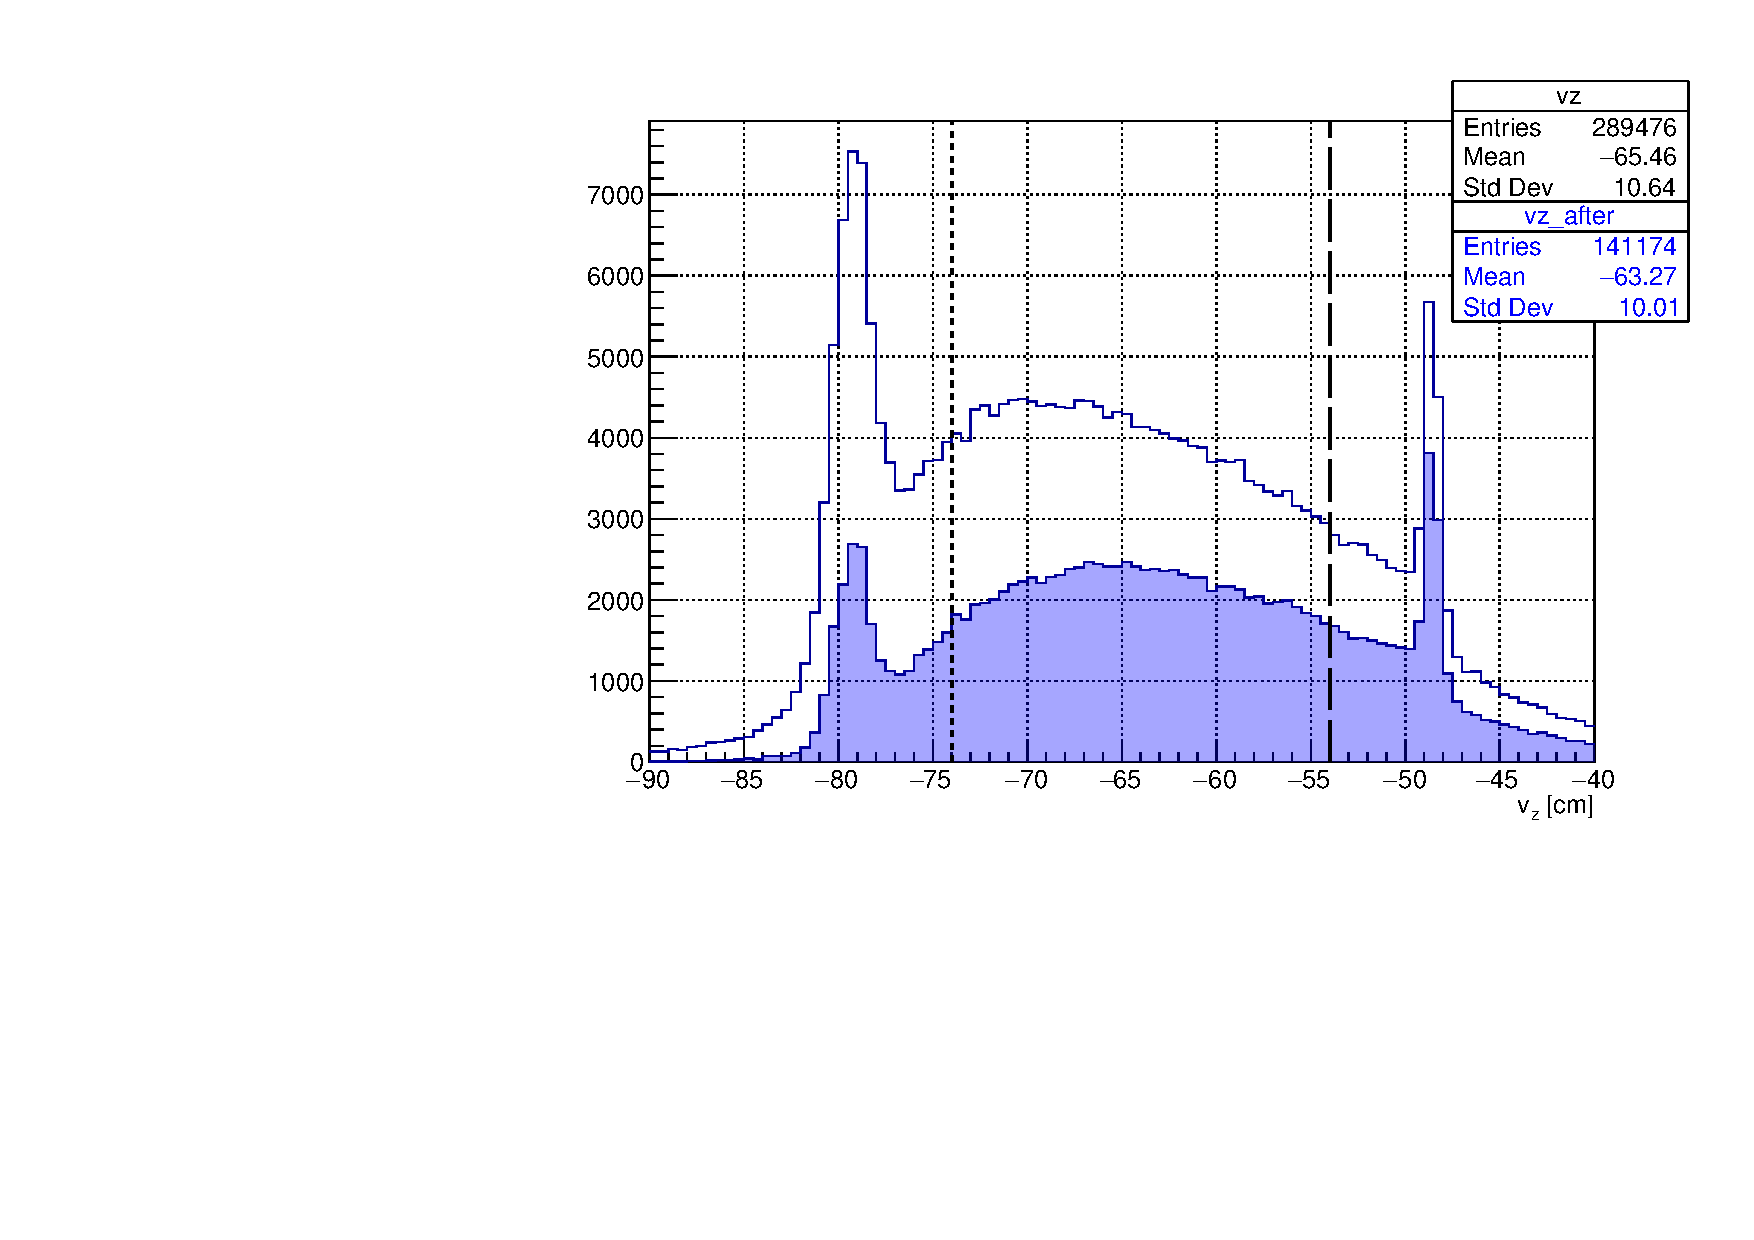
\includegraphics[width=0.5\textwidth]{figs/pid/e/pdf/vz_good}
          \caption[...]{Vertex Cut: Only particles coming from well inside the target walls are accepted.} 
        \end{figure}
Electrons were identified using their measured momentum
%light yield, time, and 
obtained from the DC, 
%Cˇerenkov counters, scintillator counters, 
and energy from the EC. The electrons were made sure to have come from within the target walls using a vertex cut.
To ensure the electrons were not low momentum \moller electrons, a momentum cut was used. 
To make sure the electrons were not minimally ionizing $\pim$, a cut on the deposited EC energy was made. 
A series of fiducial cuts were also made to make sure that all detected electrons were measured within the sensitive parts of 
the detectors.
        \begin{figure}[h!]
          \centering
          \captionsetup{width=\linewidth}
            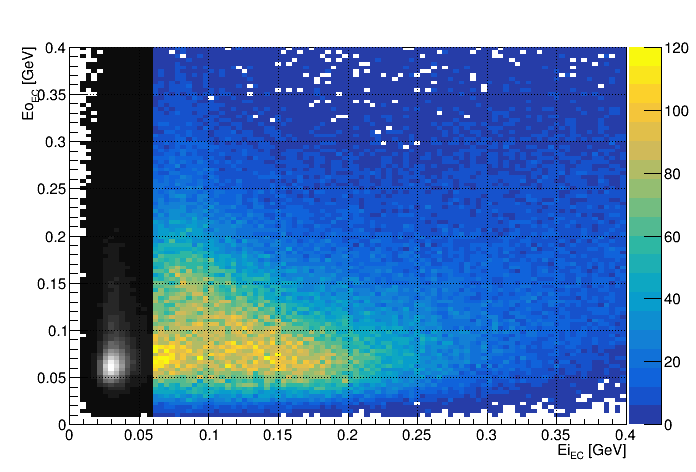
\includegraphics[width=0.5\textwidth]{figs/pid/e/ec_EOvEI.png}
          \caption[...]{EC Energy Cut: The minimum ionizing $\pi^-$ imprint can be seen in grayscale are rejected.} 
          \label{fig:pid:e:ec_e}
        \end{figure}

        \begin{figure}[h!]
          \centering
          \captionsetup{width=\linewidth, format=hang}
            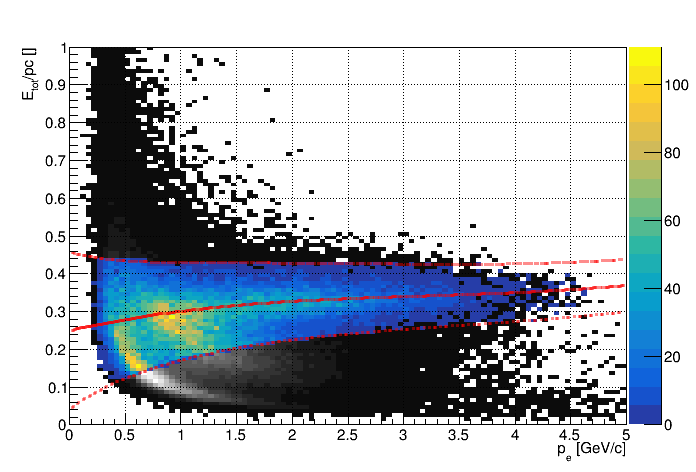
\includegraphics[width=0.5\textwidth]{figs/pid/e/ec_SFvP.png}
            %\\
            \caption[...]{EC Sampling Fraction Cut: The distributions of the energy and sector dependent EC sampling fraction as a function of momentum are shown (for sector 1). The dependence is fitted and measurements 3.5 $\sigma$ outside the fit are rejected (shown in red).} 
            \label{fig:pid:e:ec_sf}
        \end{figure}
%%%%%%%%%%%%%%%%%%%%%%%%%%%%%%%%%%%%%%%%%%%%%%%%%%
\subsection{Helium Identification}
%%%%%%%%%%%%%%%%%%%%%%%%%%%%%%%%%%%%%%%%%%%%%%%%%%
        \begin{figure}[h!]
          \centering
            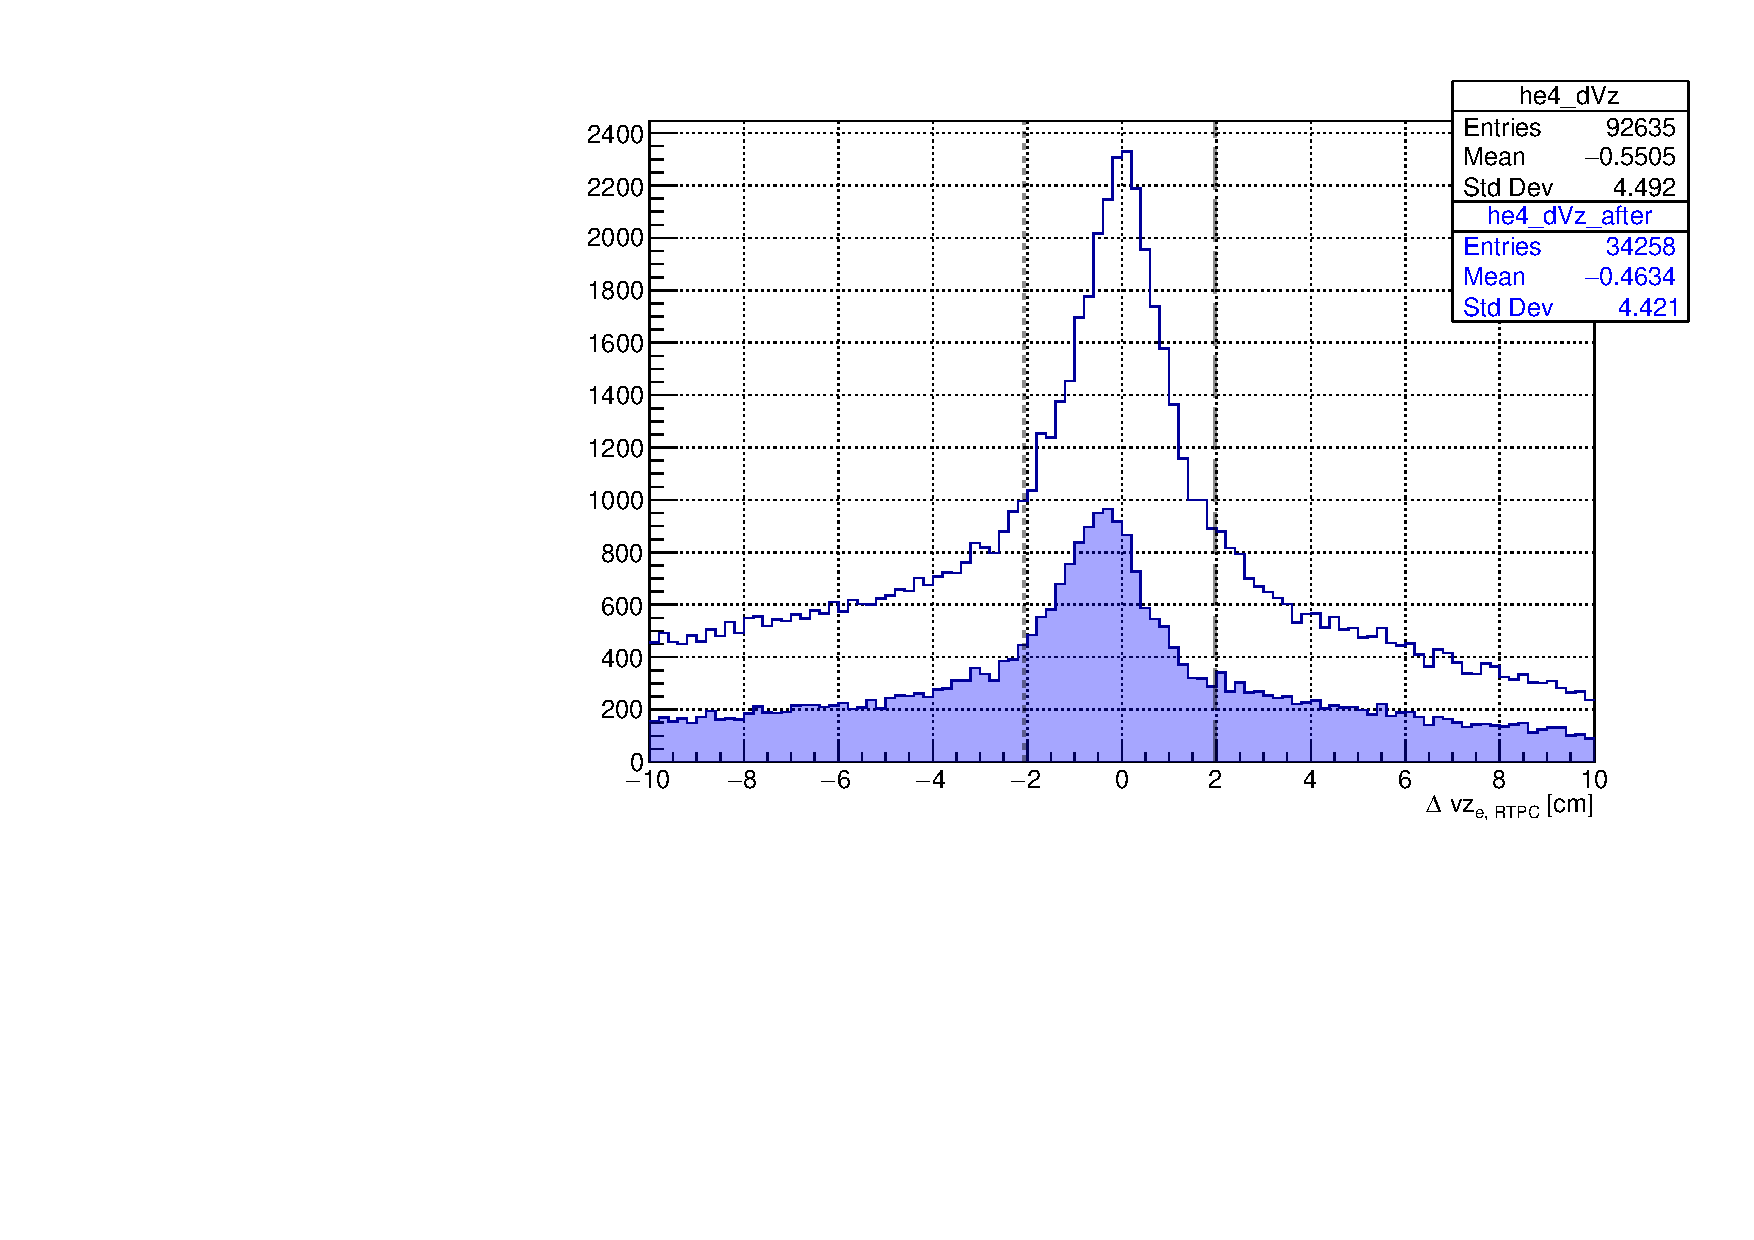
\includegraphics[width=0.5\textwidth]{figs/pid3/dVz}
            \caption[...]{Vertex Coincidence Cut: Vertices that are too far from the trigger electron are rejected.} 
            \label{fig:pid:he4:dvz}
        \end{figure}
The recoiling $\he$ nuclei were identified in the RTPC using time and energy-loss cuts for tracks in the fiducial region 
%[46]
. 
The $\he$ were selected so that the tracks were to be well within the drift region of the RTPC.
In addition, a vertex-matching cut to was applied to ensure that the electron and helium nucleus originated from a common reaction vertex in the target cell. 
%%%%%%%%%%%%%%%%%%%%%%%%%%%%%%%%%%%%%%%%%%%%%%%%%%
\subsection{Photon Identification}
%%%%%%%%%%%%%%%%%%%%%%%%%%%%%%%%%%%%%%%%%%%%%%%%%%
        \begin{figure}[h!]
          \centering
          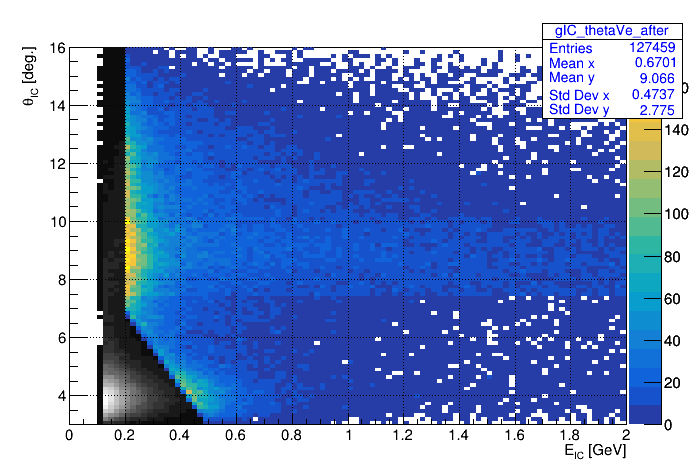
\includegraphics[width=0.5\textwidth]{figs/pid/g/IC/thetaVe}
          \caption[...]{\moller Electron Cut: A geometric cut is applied to reject low-energy, low-angle \moller electrons} 
          \label{fig:pid:gic:moller}
        \end{figure}
The photons were detected in either the IC or the CLAS electromagnetic calorimeters. Note that even though the DVCS reaction has only one real photon in the final state, events with more than one good photon were not discarded at this stage. These were mainly caused by accidental coinci- dences of soft photons and did not directly affect this measurement, as only the most energetic photon of an event was considered a DVCS photon candidate. This prescription however slightly increased the corrections associated with the π0 and the accidental backgrounds discussed below.

%%%%%%%%%%%%%%%%%%%%%%%%%%%%%%%%%%%%%%%%%%%%%%%%%%%%%%%%%%%%%%%%%%%%%%%%%%%%%%%%%%%%%%%%%%%%%%%%%%%%
\section{Event Selection \label{kinfit}}
%%%%%%%%%%%%%%%%%%%%%%%%%%%%%%%%%%%%%%%%%%%%%%%%%%%%%%%%%%%%%%%%%%%%%%%%%%%%%%%%%%%%%%%%%%%%%%%%%%%%
The detection of a scattered electron, a recoiled helium track, and two photons alone does not mean that the event is part of the exclusive coherent $\dvmp$ off $\he$. Any one of the detected particles could be misidentified and any subset of the particles detected could be part of an entirely different process. Event selection is required to sort through these sets of particles to select the relevant coherent $\dvmp$ process.
%%%%%%%%%%%%%%%%%%%%%%%%%%%%%%%%%%%%%%%%%%%%%%%%%%%
%\subsection{Kinematic Fitting}
%%%%%%%%%%%%%%%%%%%%%%%%%%%%%%%%%%%%%%%%%%%%%%%%%%%

\subsection{Kinematic Fitting}
Kinematic fitting leverages hard physical constraints with soft uncertainties (and pairwise correlations) in measurement. That is, fitted values are guided by constraints (e.g. conservation of momentum and energy) to move within the measurement uncertainies, to simultaneously improve the measured values. 

For coherent $\dvmp$, the simultaneous constraints of conservation of energy and momentum for the exclusivity (4 constraint equations) of 
\begin{align*}
  \coherent 
\end{align*}
and the decay of the $\pio$ into two photons (4 constraint equations)
\begin{align*}
  \decay  \quad,
\end{align*}
provides 8 total constraint equations. 
Since the $p, \theta$ and $\phi$ of $\pio$ are not directly measured, the fit is a $5C$ fit.

An approximate covariance matrix was used and both the confidence level distribution and, for a 5\% confidence level cut (CLC), the pull distributions were reasonably expected.
\begin{figure}[h!]
    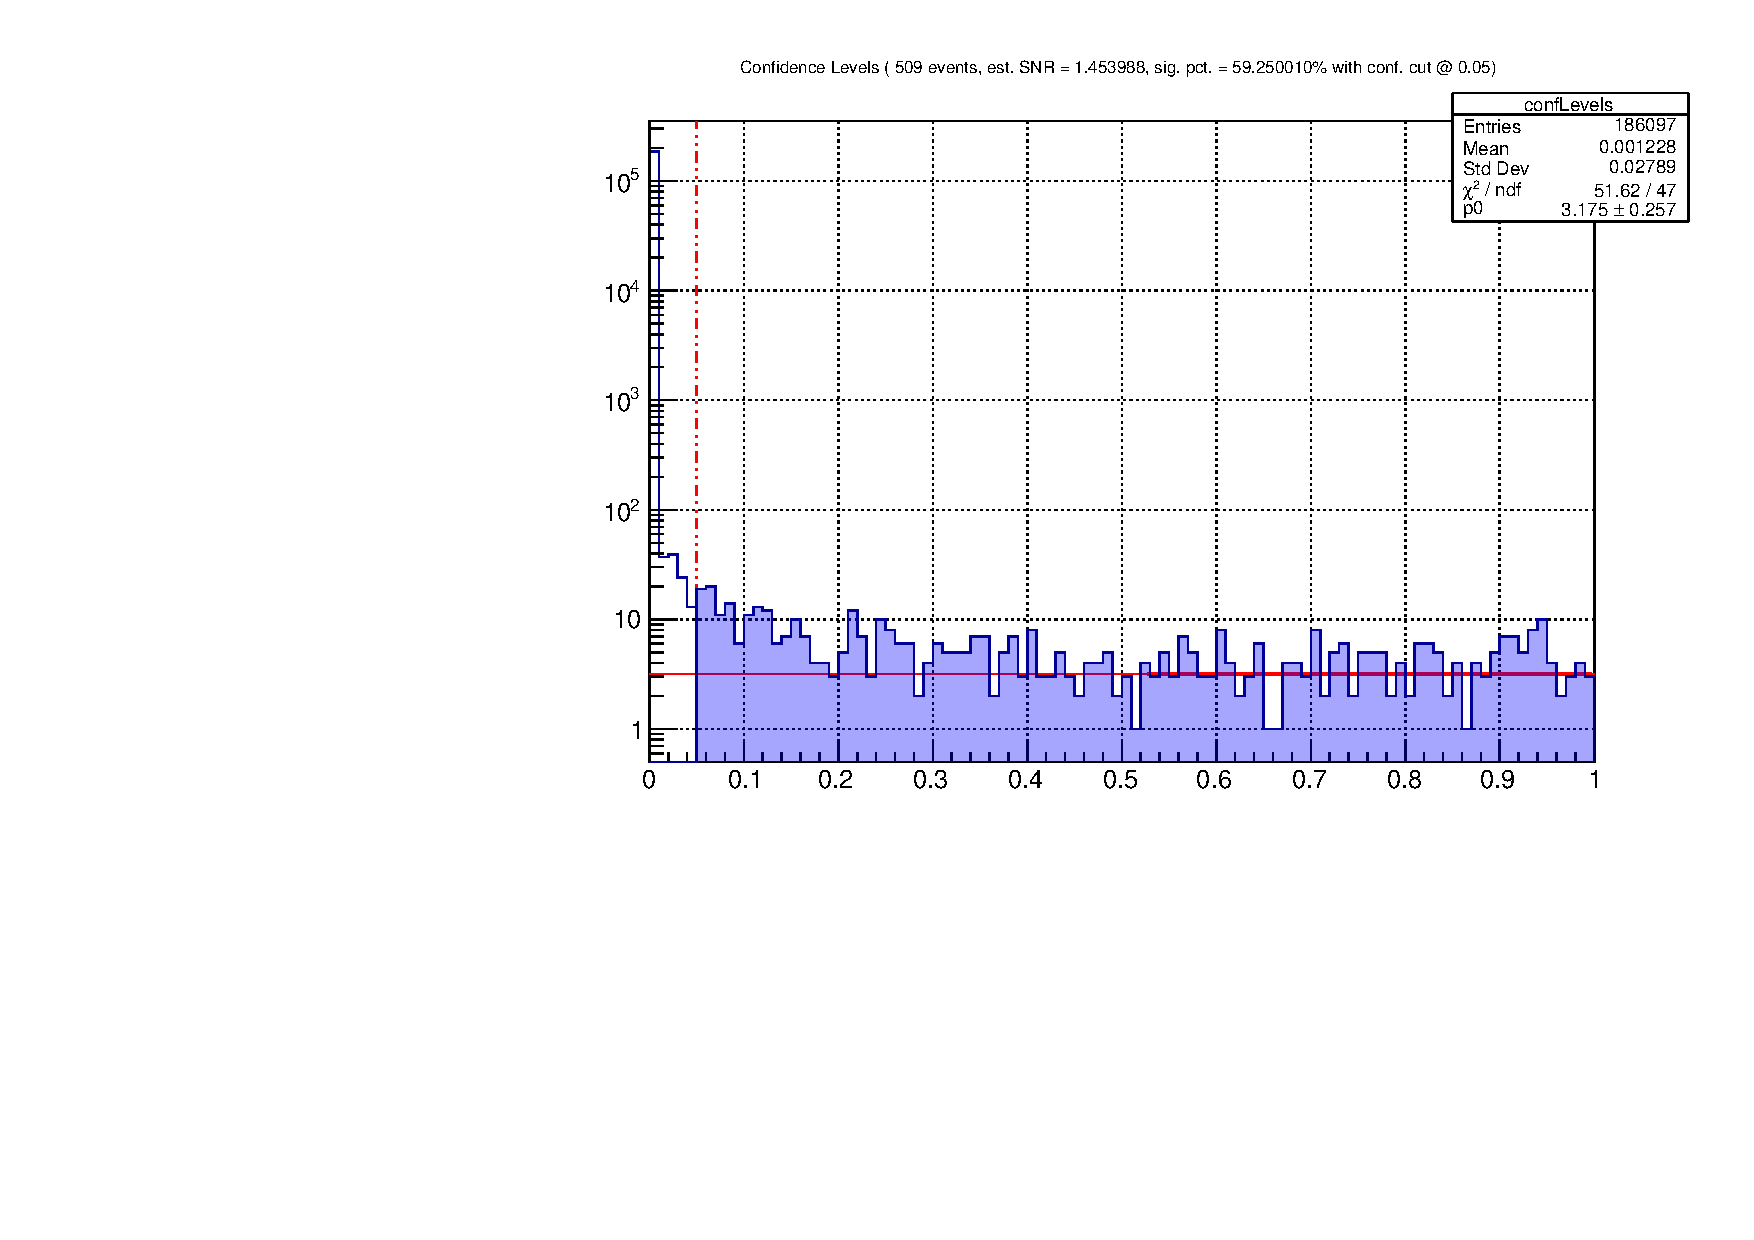
\includegraphics[width = 0.5\textwidth]{figs/coh_pi0/confLevels.pdf}
    \caption{Confidence level of $5C$ kinematic fit with a 5\% confidence level cut applied. \\Events selected are highlighted blue. }
    \label{cl}
\end{figure}
\begin{figure}
    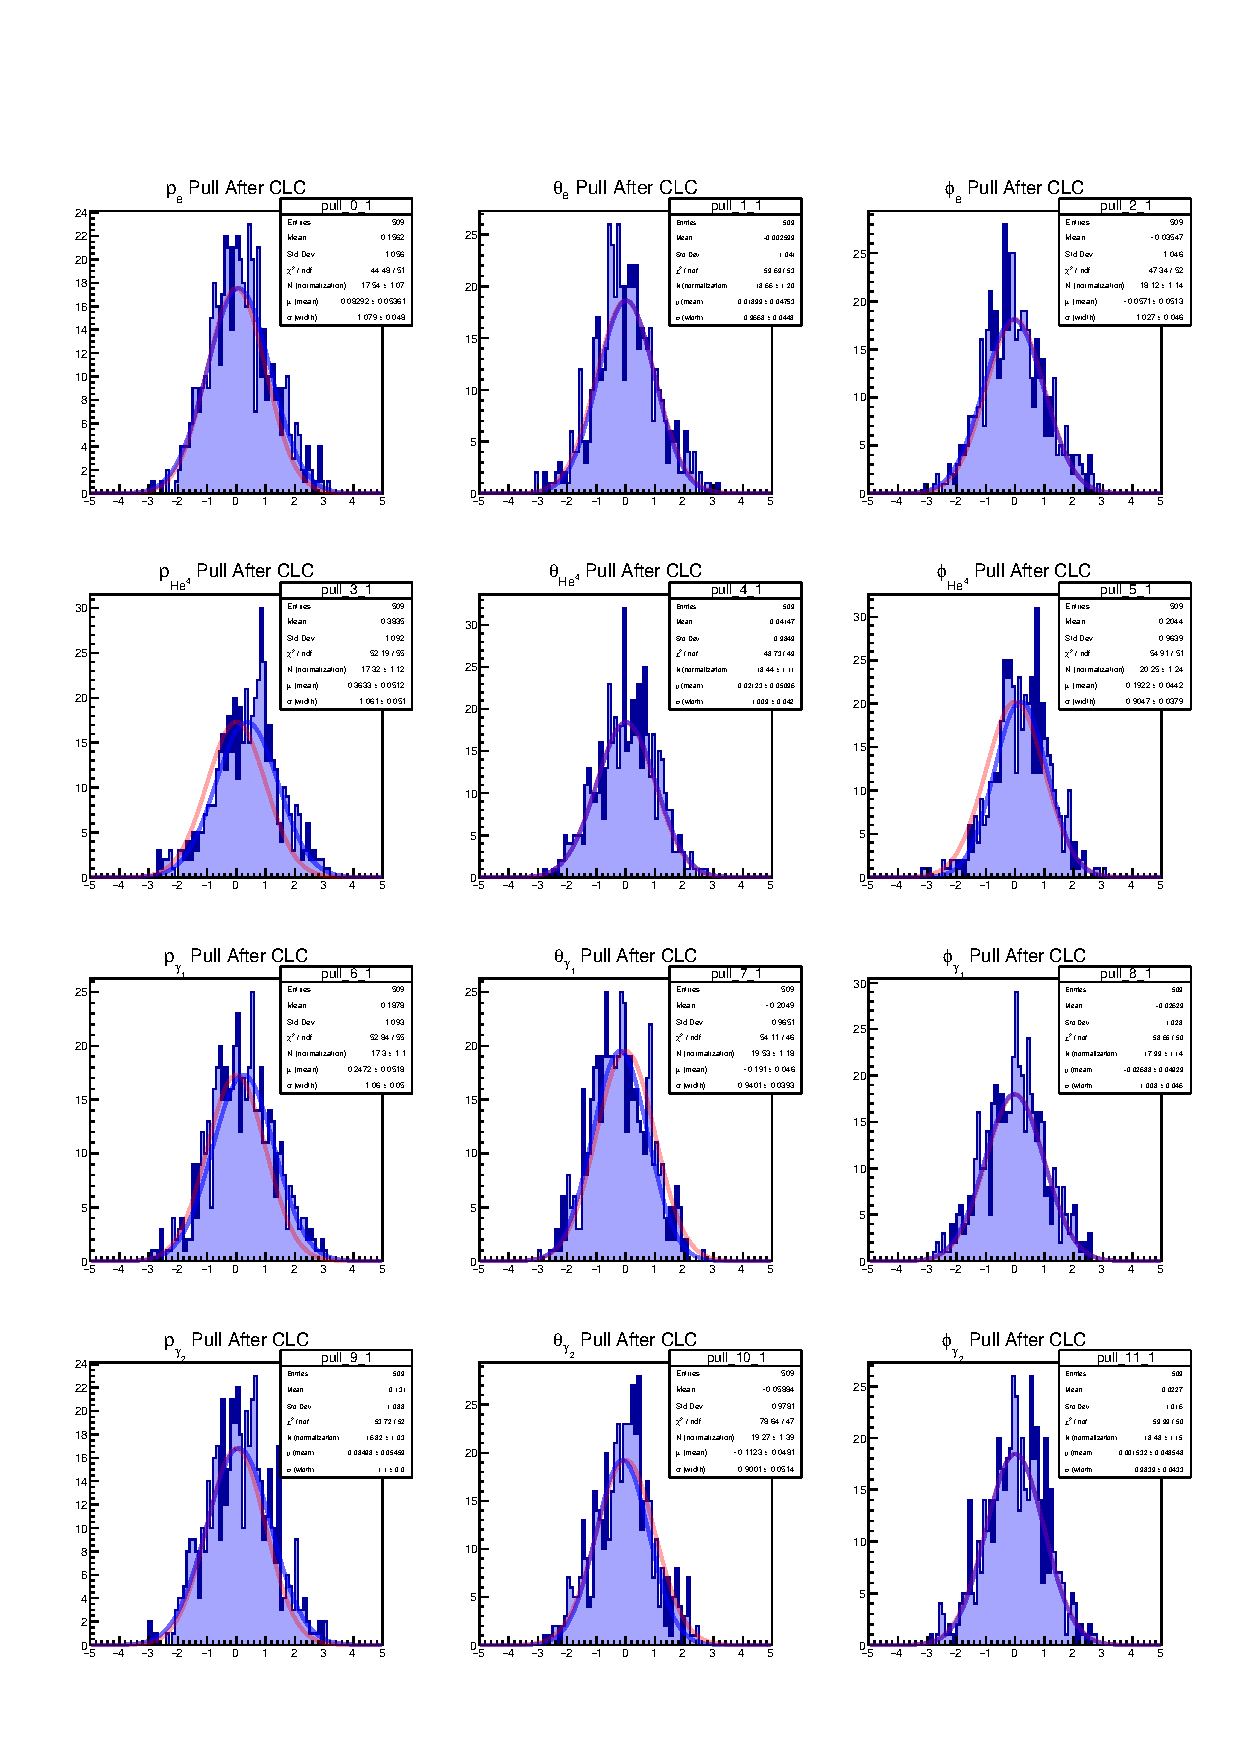
\includegraphics[width = 0.5\textwidth]{figs/coh_pi0/pulls.pdf}
    \caption{Pull disitrbutions of $5C$ kinematic fit selected with a 5\% confidence level cut (highlighted in blue). The events selected are fit to a Gaussian (blue curve) and are compared to what they are expected to be (in red). \label{pulls}}
\end{figure}

%%%%%%%%%%%%%%%%%%%%%%%%%%%%%%%%%%%%%%%%%%%%%%%%%%
\subsection{Exclusivity Variable Distributions}
%%%%%%%%%%%%%%%%%%%%%%%%%%%%%%%%%%%%%%%%%%%%%%%%%%
%%%%%%%%%%%%%%%%%%%%%%%%%%%%%%%%%%%%%%%%%%%%%%%%%%
It is also useful to look at the resulting exclusivity variable distributions obtained from the $5C$-fit with CLC at 0.05.  
These distributions give a qualitative feel of whether the particles selected are a part of an exclusive process. 
The distributions of the selected events are shown in \Fig{\ref{figs:kinfit:5C:carts}}, from left to right respectively, with
\begin{itemize}
  \item 
  the top row being the missing mass$^2$ distributions for the 
  \begin{itemize}
    \item the missing $\he$ ($e ~\he \rightarrow e ~\pio$), 
    \item the missing $\pio$ ($e ~\he \rightarrow e ~\he$), and 
    \item the full exclusivity ($e ~\he \rightarrow e ~\he ~\pio$) .
  \end{itemize}
  \item 
  the middle row being the missing $x$, $y$, and transverse momentum components from the full exclusivity,
  \item 
  and the bottom row being 
  \begin{itemize}
    \item the missing energy, $E$, from the full exclusivity; 
    \item the angle between the missing and measured $\pio$ 3-momentum, $\theta$; and 
    \item the angle between the plane formed by the virtual photon and the initial $\he$ and the plane formed by the initial and finial state $\he$.
  \end{itemize}
  \end{itemize}
%Again, despite the similar distributions, the measured variables passing the kinematic fit (blue) have tails that are suppresed as compared to the ones passing the exclusivity cuts (black).

  These distributions along with the photon pair invariant mass distribution give a great degree of confidence in the selected events belonging to the exclusive coherent $\pio$ production process: $e ~\he \rightarrow e ~\he ~\pio$. With these selected events, the beam spin asymmetry for this process can be extracted.
  \clearpage
  \begin{figure}[h!]
    \centering
    \captionsetup{width=\linewidth, format = hang}
    %\includegraphics[width=0.78\textwidth]{figs/5C/carts}
    %\includegraphics[width=\textwidth]{figs/5C/carts}
    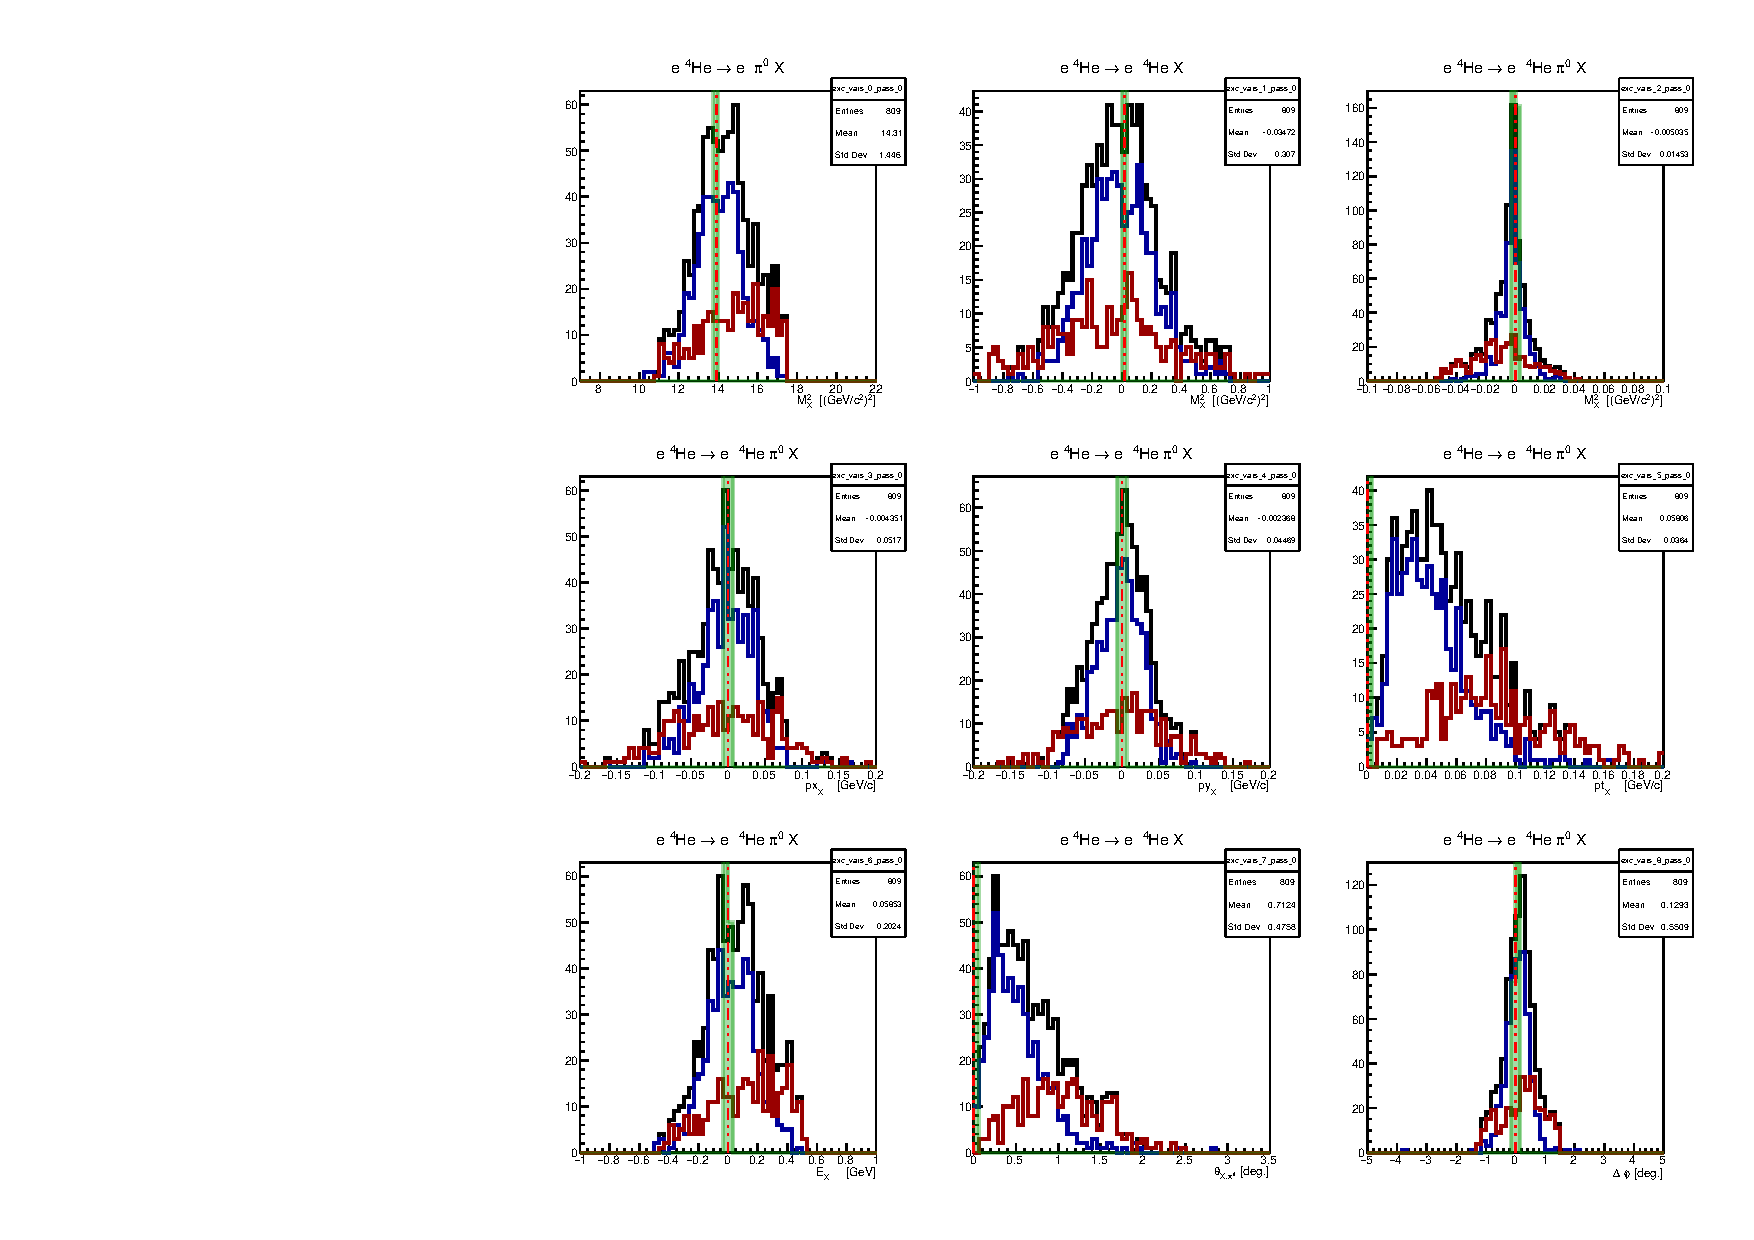
\includegraphics[width=0.5\textwidth]{figs/new_algo/with_clc/exc_vars}
    \caption[...]{ Exclusivity variable distributions for: \\
      \qquad - Measured events passing exclusivity cuts (black) \cite{torayev}\\
      \qquad - Measured events passing kinematic fit with 0.05 CLC (blue)  \\
      \qquad - Fitted events   passing kinematic fit with 0.05 CLC (highlighted green) \\
      \qquad - Measured events failing kinematic fit with 0.05 CLC but passing exclusivity cuts (red)  \\
      with the expected values indicated by the vertical red dashed line.
      }
    \label{figs:kinfit:5C:carts}
  \end{figure}


%%%%%%%%%%%%%%%%%%%%%%%%%%%%%%%%%%%%%%%%%%%%%%%%%%
\section{Kinematic Binning}
%%%%%%%%%%%%%%%%%%%%%%%%%%%%%%%%%%%%%%%%%%%%%%%%%%
Since the events selected are very limited (see \Fig{\ref{fig:kin_binning}}), there was one combined kinematic bin in $Q^2$, $x$, and $t$. From there, we can extract the variation in $\phi$ of the beam spin asymmetry by binning $\phi$ into a few bins.  
%\begin{figure*}
%  \subfloat[text for the first subfigure\label{sfig:testa}]{
%    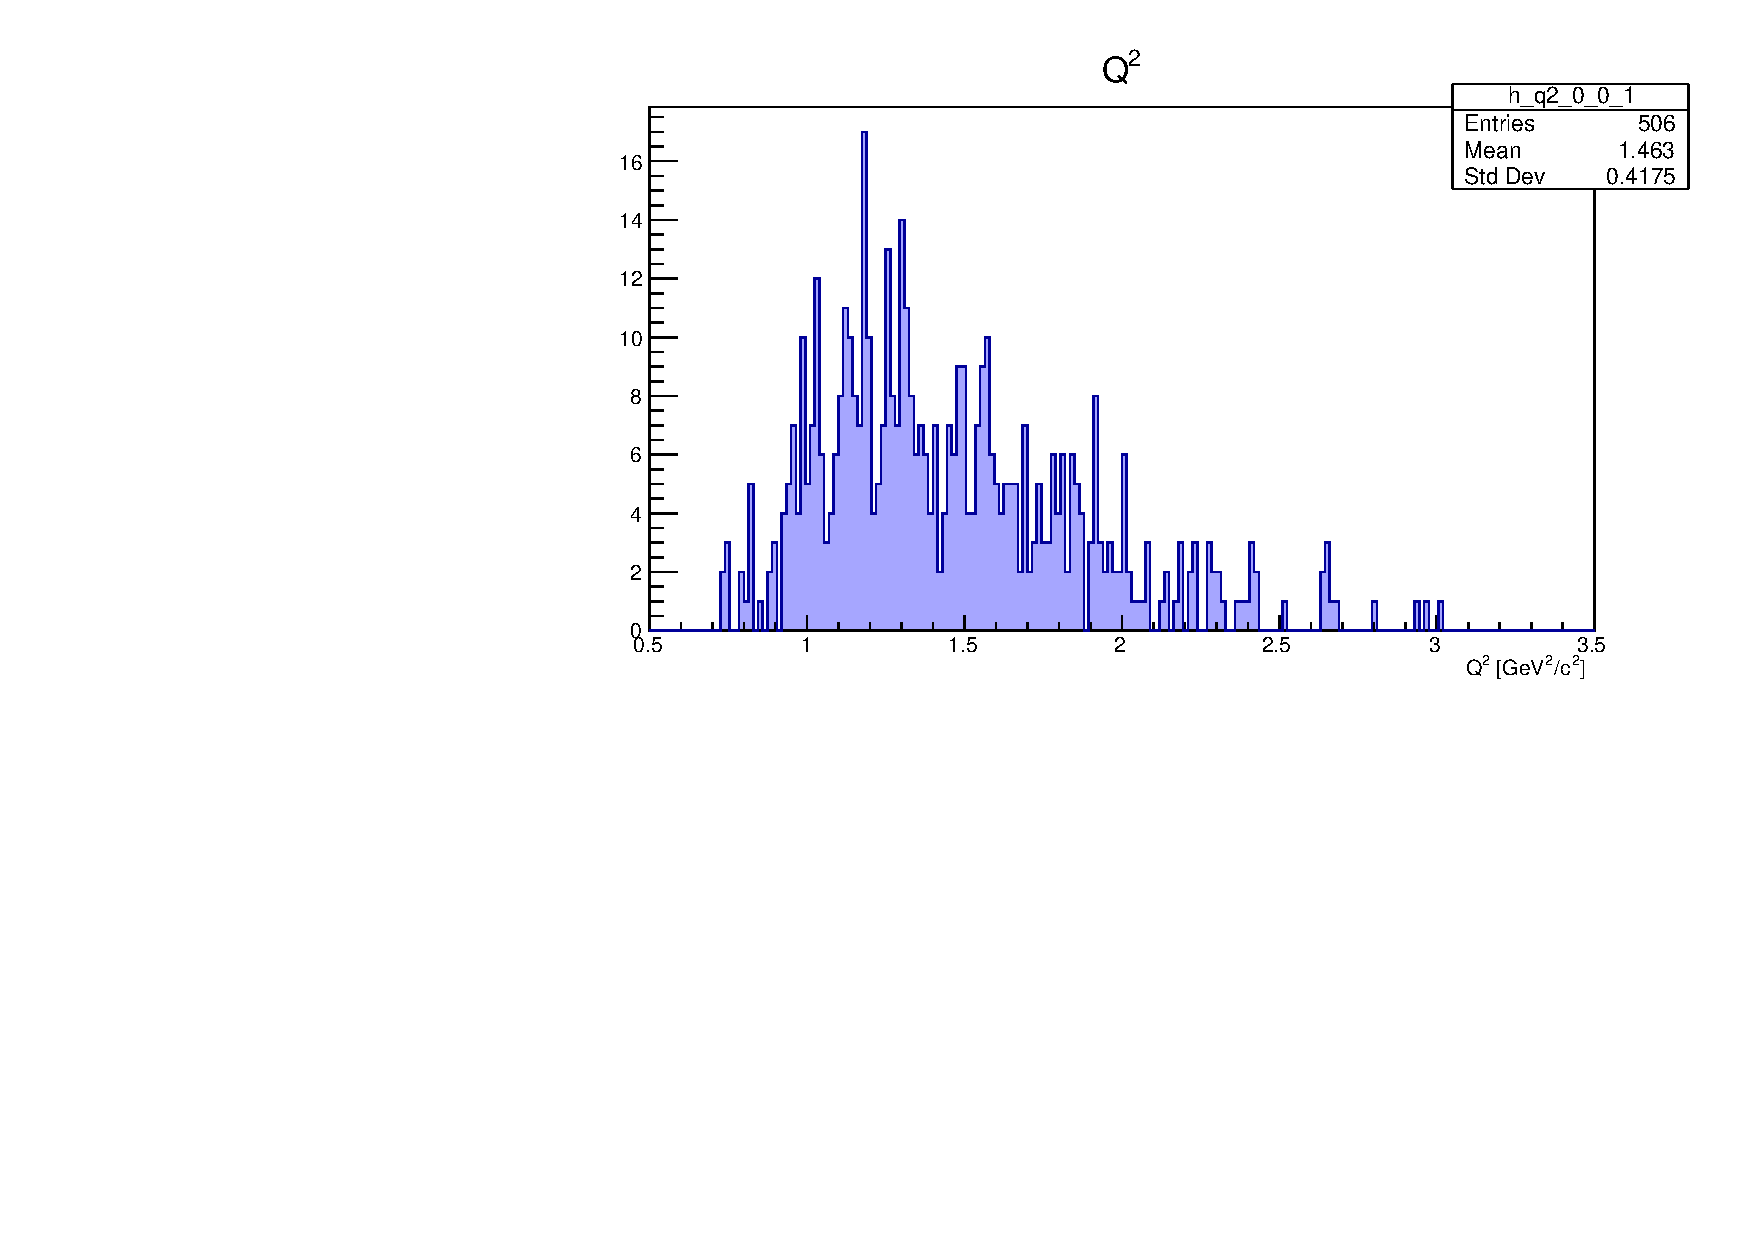
\includegraphics[trim={0  0 0 19.75px},clip, width = \textwidth]{figs/coh_pi0/binning_Q2}
%  }
%\subfloat[text for the second subfigure\label{sfig:testa}]{%
%  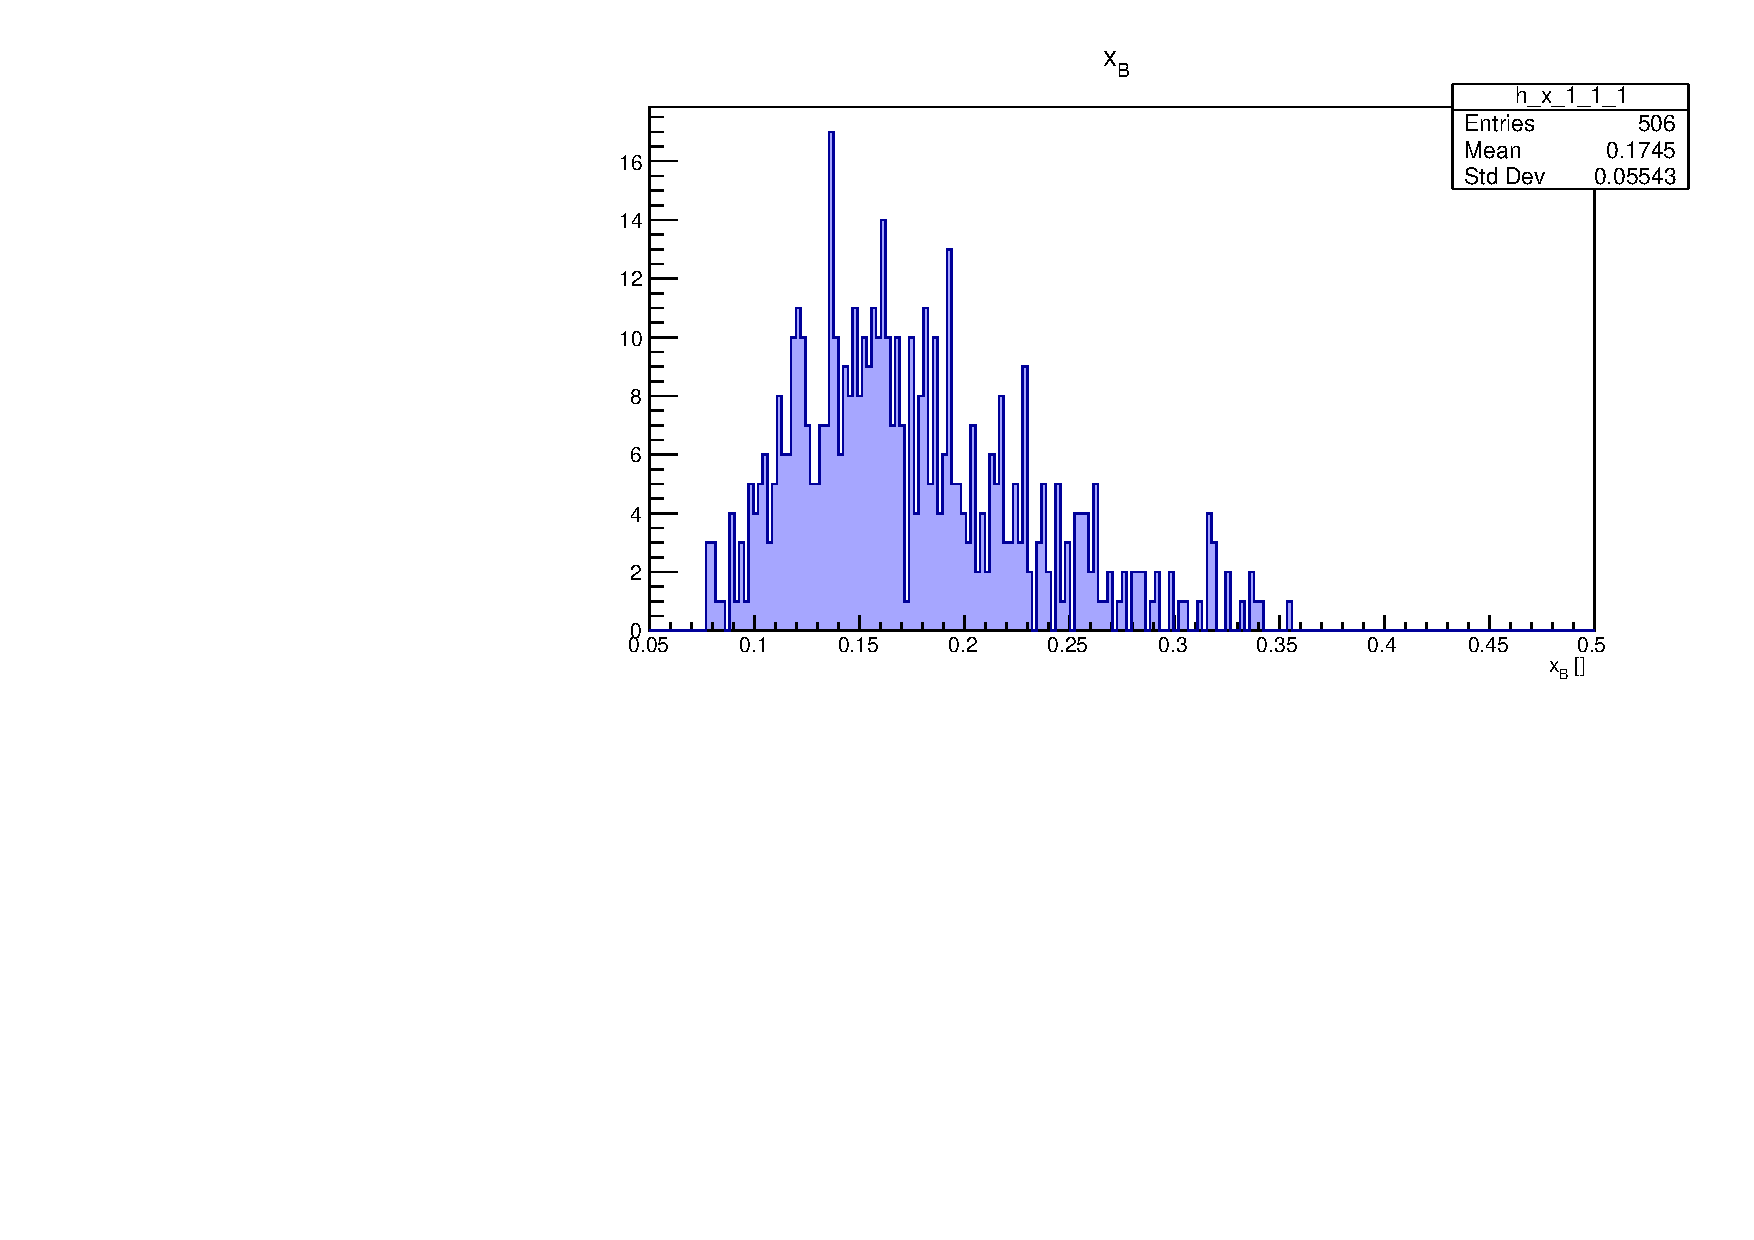
\includegraphics[trim={0  0 0 19.75px},clip, width = \textwidth]{figs/coh_pi0/binning_x}
%}
%\caption{}
%\label{}
%\end{figure*}
\begin{widetext}
\begin{figure*}
\subfloat{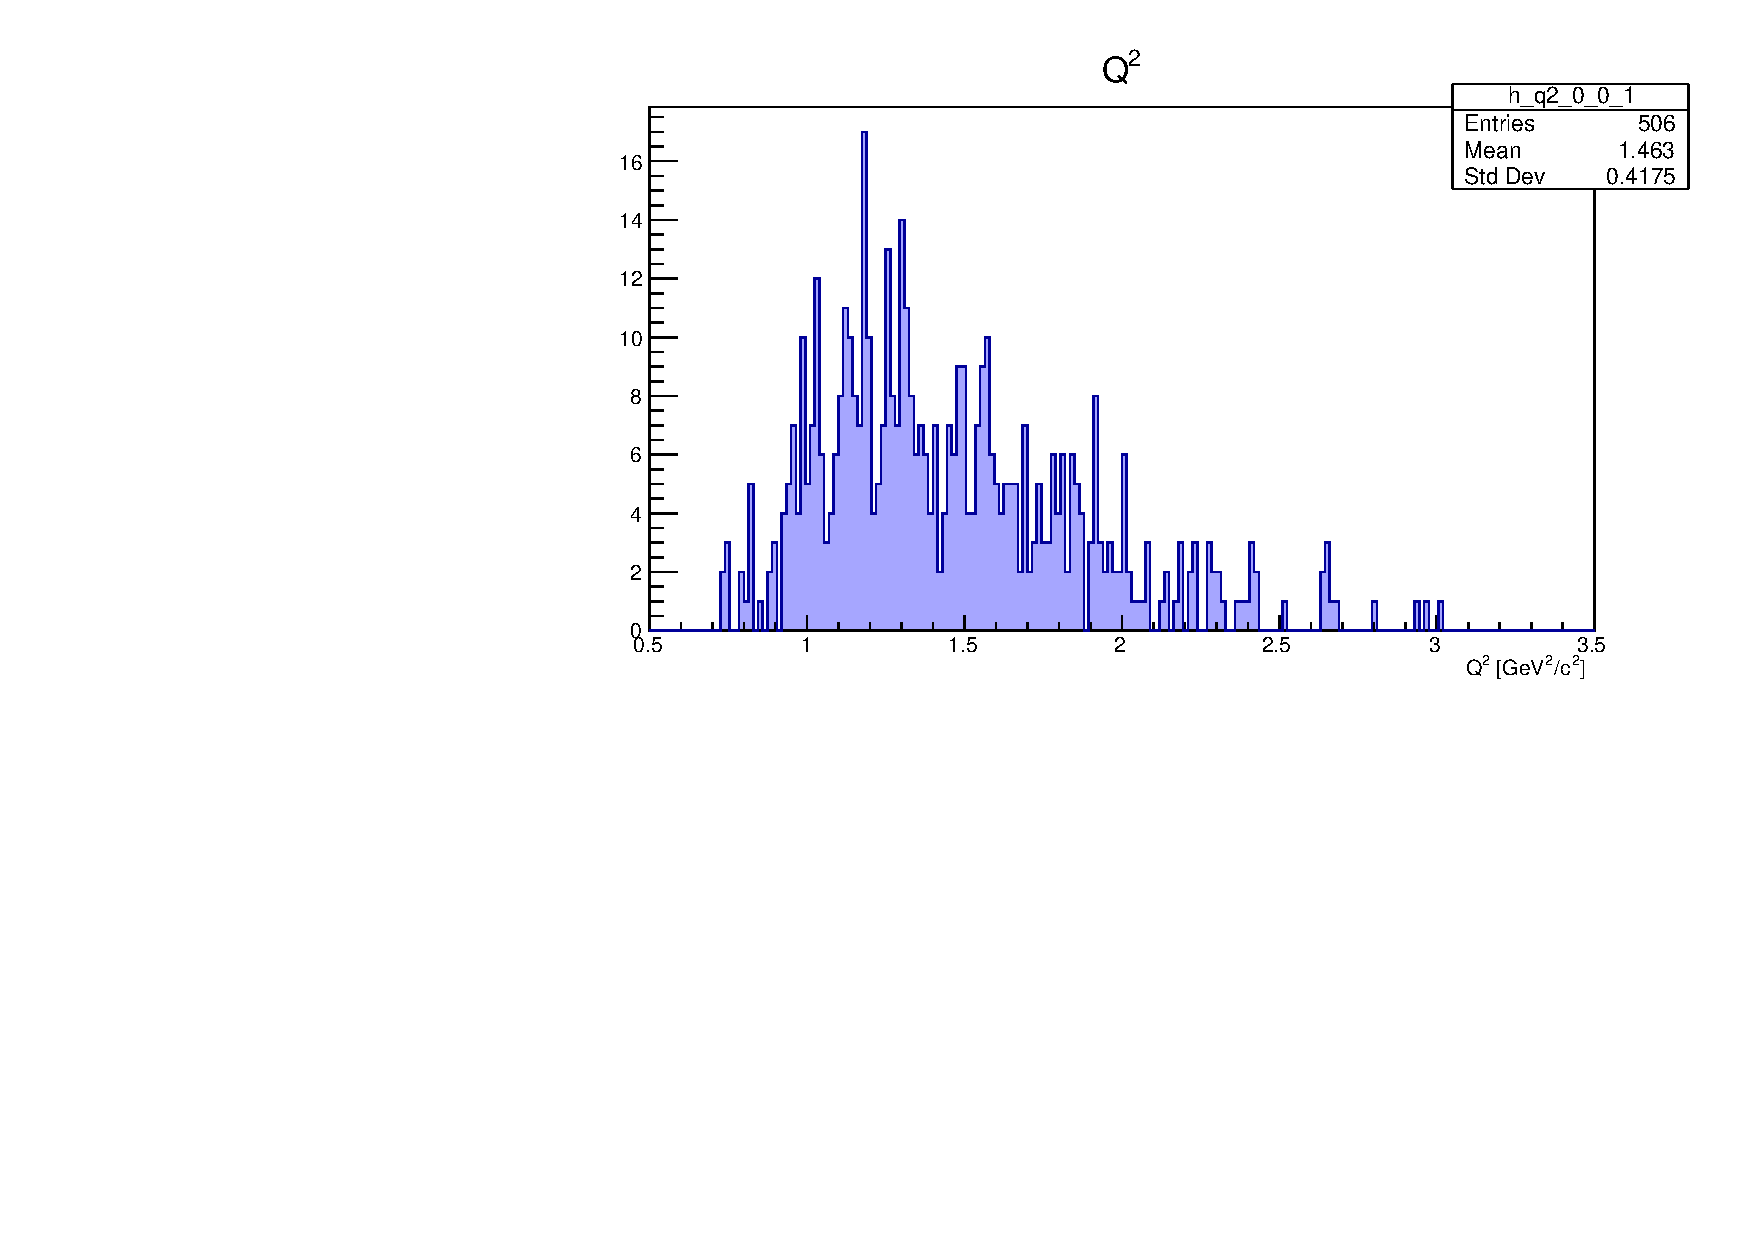
\includegraphics[trim={0  0 0 19.75px},clip, width=0.25\textwidth]{figs/coh_pi0/binning_Q2} }
\subfloat{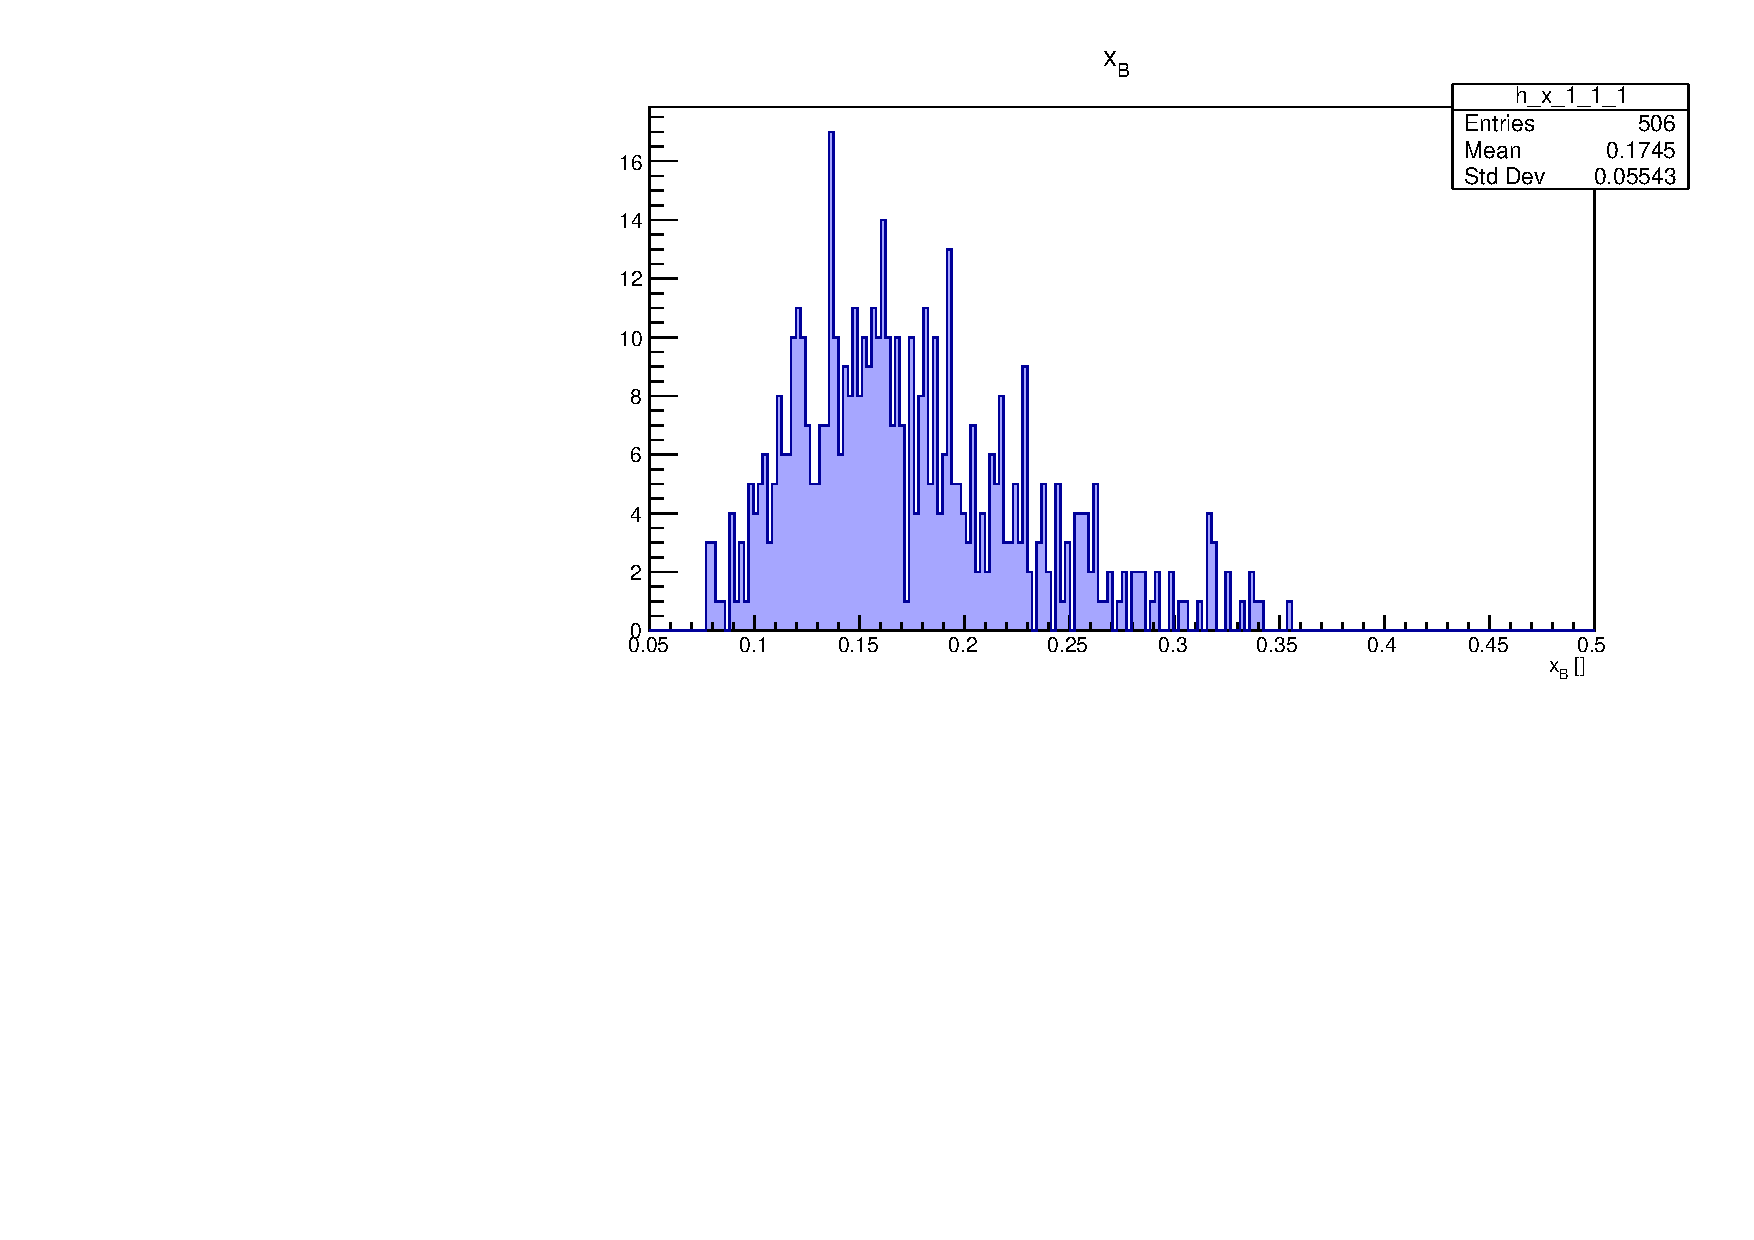
\includegraphics[trim={0  0 0 19.75px},clip, width=0.25\textwidth]{figs/coh_pi0/binning_x} }
\subfloat{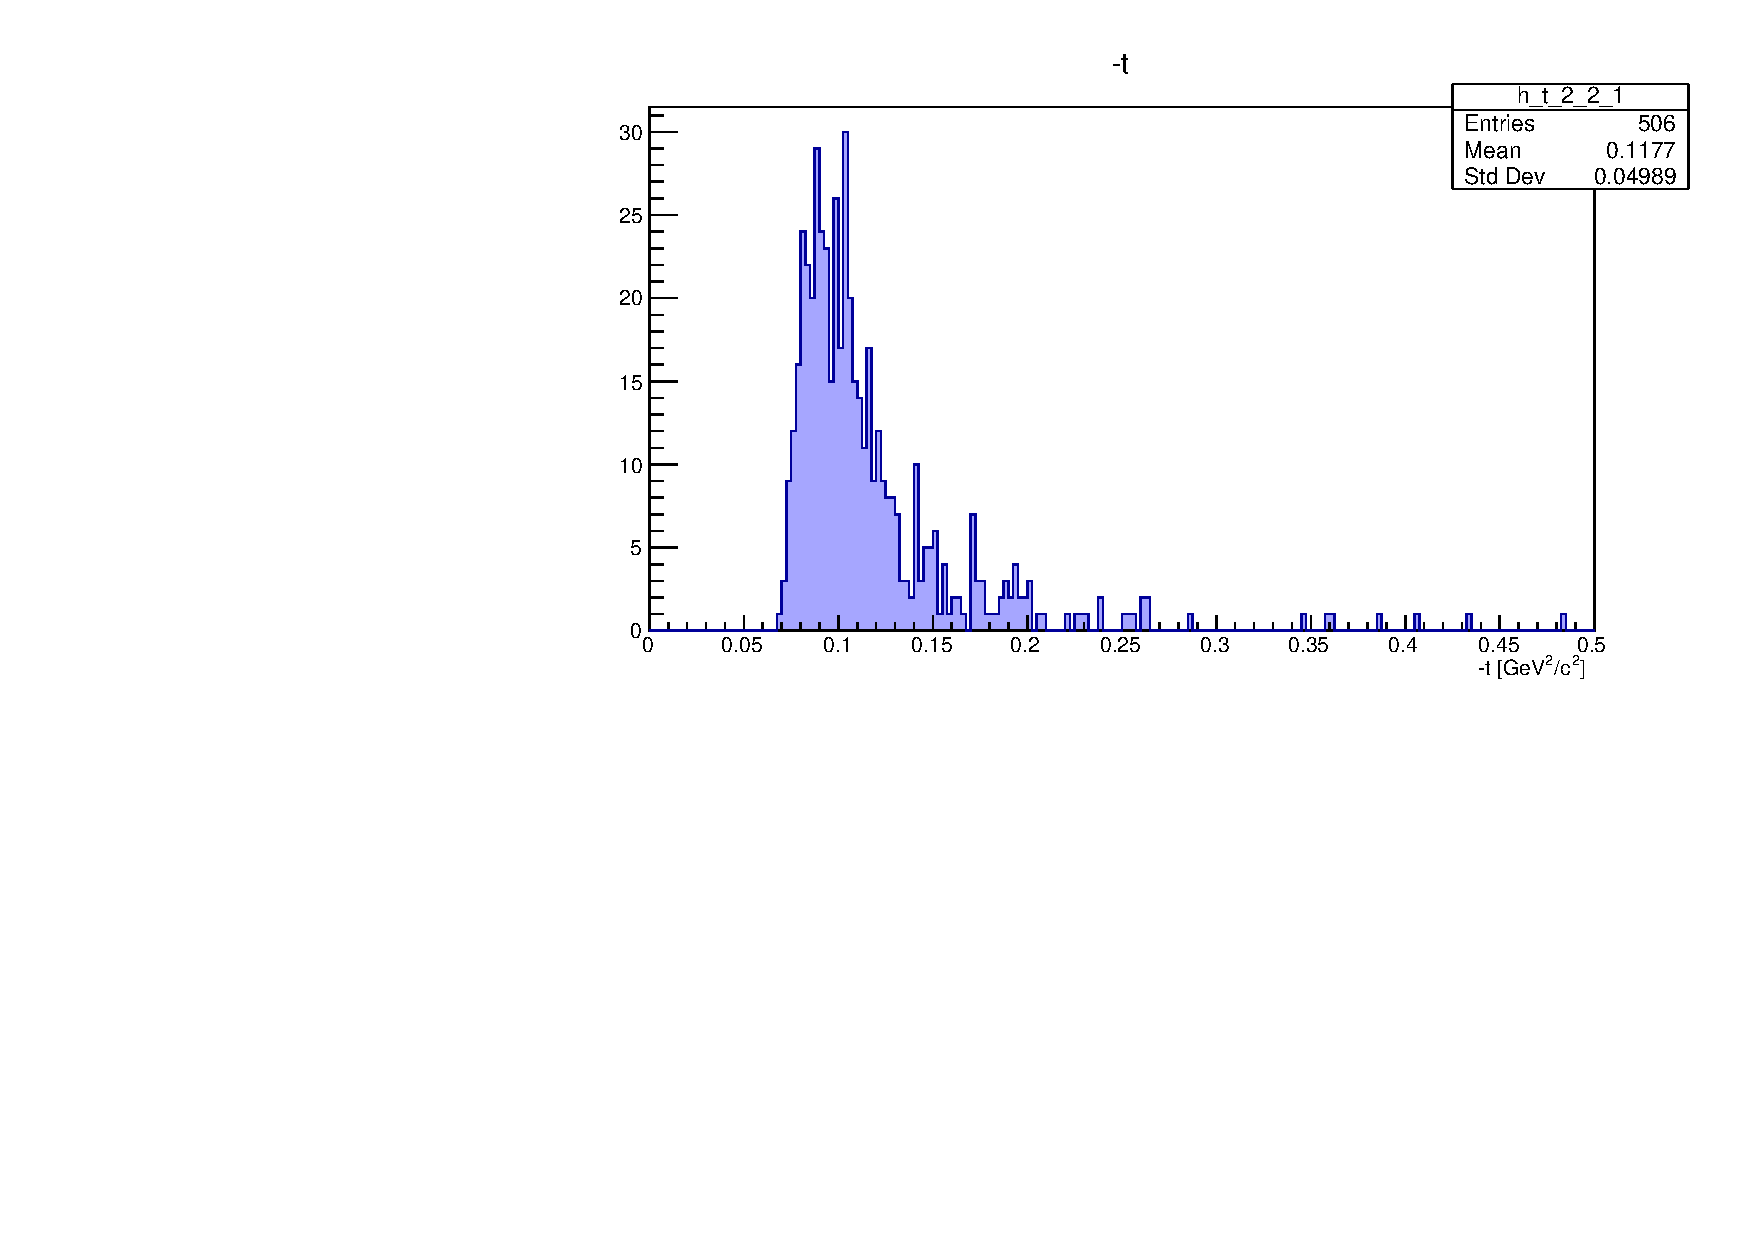
\includegraphics[trim={0  0 0 19.75px},clip, width=0.25\textwidth]{figs/coh_pi0/binning_t} }
\subfloat{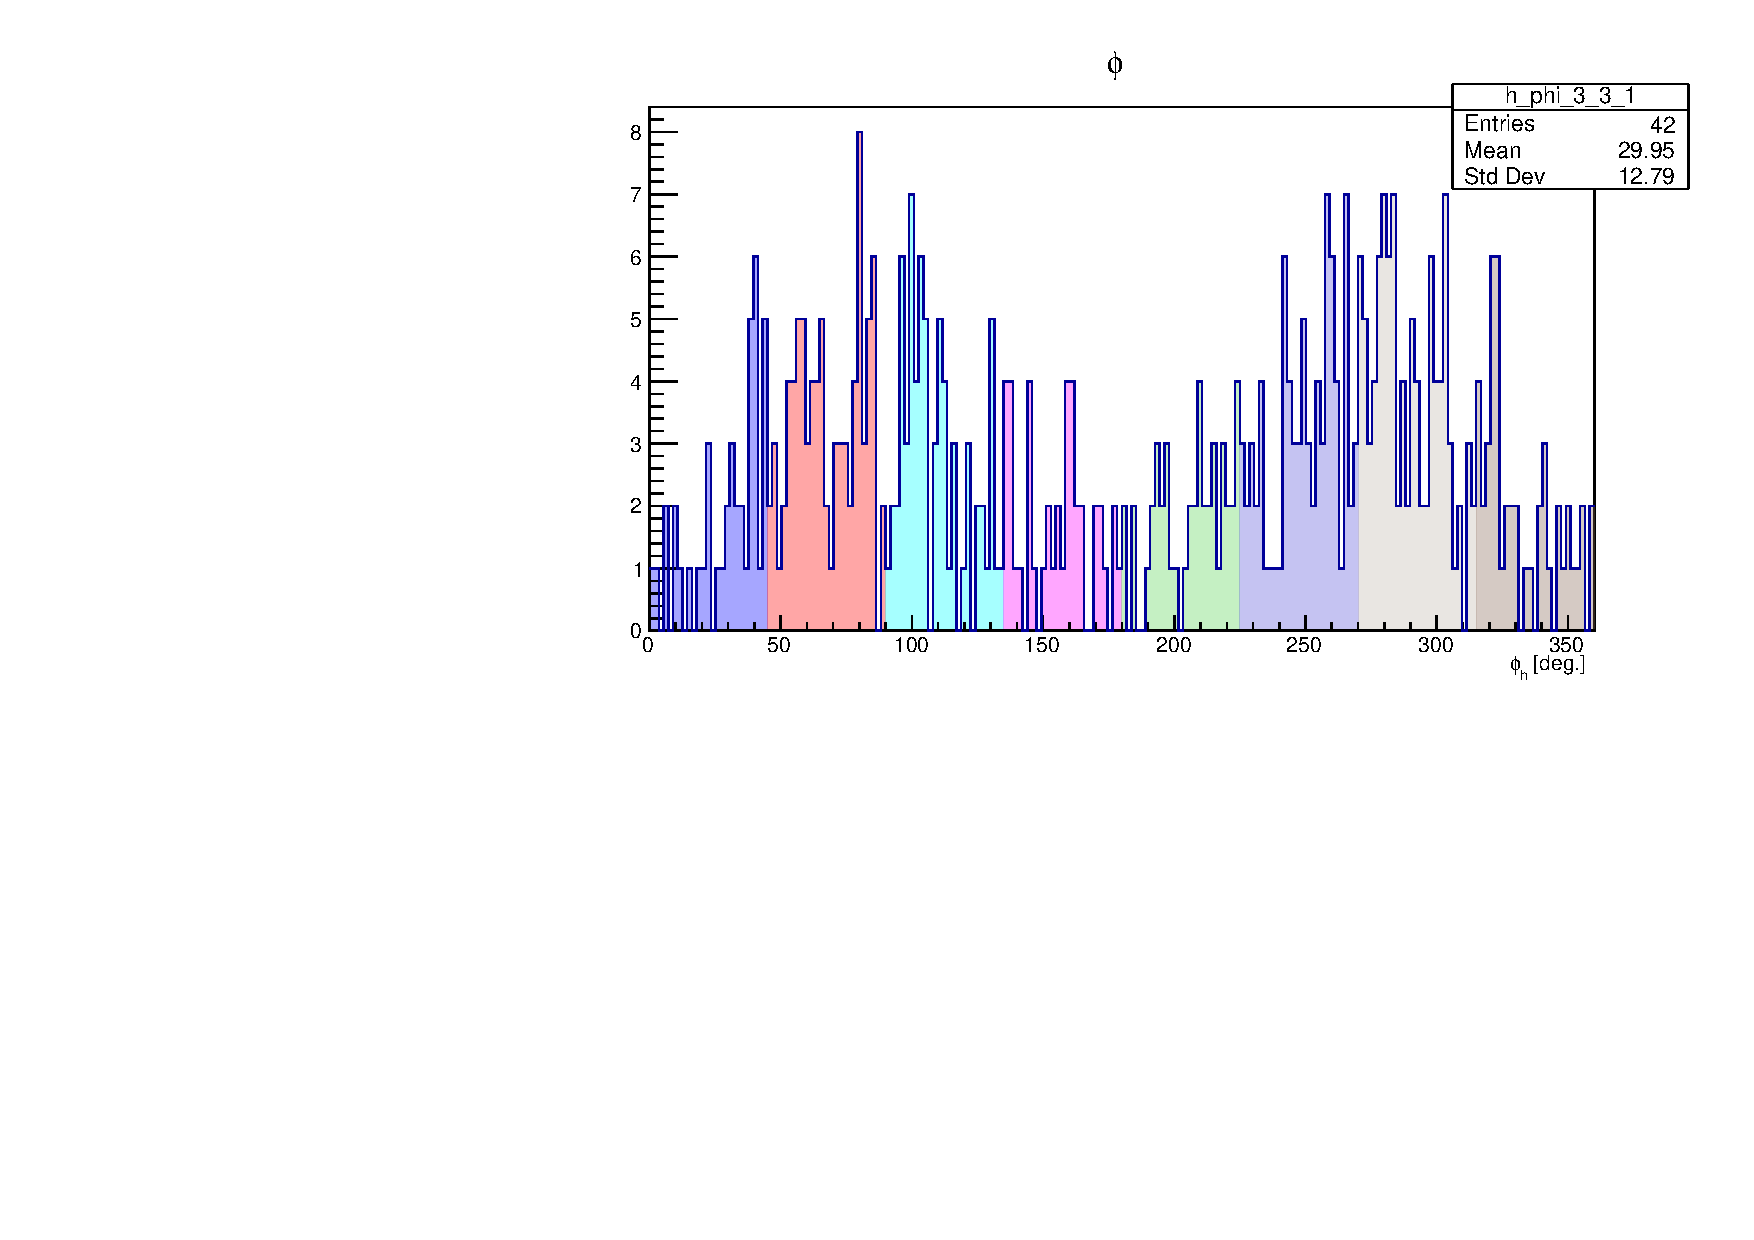
\includegraphics[trim={0  0 0 19.75px},clip, width=0.25\textwidth]{figs/coh_pi0/binning_phi} }
\caption{Kinematic binning in $Q^2, x, -t$ and $\phi$, respectively.}
\label{fig:kin_binning}
\end{figure*}
\end{widetext}

$Q^2$, $x$, and $t$ form a single kinematic bin that is partitioned into 8 equally spaced $\phi$ bins to extract the beam spin asymmetry (as demarcated by color).

%%%%%%%%%%%%%%%%%%%%%%%%%%%%%%%%%%%%%%%%%%%%%%%%%%%%%%%%%%%%%%%%%%%%%%%%%%%%%%%%%%%%%%%%%%%%%%%%%%%%
\section{Systematic Uncertainties \label{systematics}}
%%%%%%%%%%%%%%%%%%%%%%%%%%%%%%%%%%%%%%%%%%%%%%%%%%%%%%%%%%%%%%%%%%%%%%%%%%%%%%%%%%%%%%%%%%%%%%%%%%%%
      \begin{table}[h!]
        \centering
        \caption{Systematic Uncertainties}
        \label{tab:sys_uncerts}
        \begin{tabular}{|c|c|c|}
          \hline
        %\multirow{2}{*}{ \begin{tabular}{c}\b{Systematic Uncertainty Source }\end{tabular}}        &\multicolumn{2}{c|}{ \begin{tabular}{c|c}\multicolumn{2}{c}{\b{Contribution}}\\\hline\end{tabular}}
        \multirow{2}{*}{ \b{Systematic Uncertainty Source }}        &\multicolumn{2}{c|}{\b{Contribution}}
             \\\cline{2-3} &$\bm{\Delta A_{LU}/A_{LU}}$  & $\bm{\Delta A_{LU}}$%  
          \\
          \hline                                                  
          %Radiative corrections               & 0.1\%             & 0.1\%         
          %\\                                                     
          Beam polarization                   & 3.50\%            & 0.04\%         
          \\                                                      
          Conf. level cut                     & --                & 2.26\%         
          \\                                                      
          $\phi$ binning                      & --                & 1.70\%         
          \\                                                      
          \hline                                                  
          \b{\u{Total}}                       & --                & 2.83\%         
          \\
          \hline
        \end{tabular}
      \end{table}
\Tab{\ref{tab:sys_uncerts}} displays a summary of the systematic uncertainties. The largest contributions to uncertainty comes from the confidence level cut and the binning of $\phi$. Although this is a study on systematics, the underlying uncertainty comes from statistics:
\begin{itemize}
  \item
    The choice of the confidence level cut comes down to maximizing statistics while minimizing background.
      \begin{itemize}
        \item
          With better statistics, a confidence level cut can be made much higher where very little background is creeping in. The nominal value chosen sits right on a steep slope of the background. Any cut higher limits the statistics dramatically and any lower increases the background noticeably.
       \end{itemize}
   \item
    The binning in $\phi$ is chosen to show if the BSA is of the form $\alpha \sin \phi$, while maintaining an appreciable amount of statistics in each bin. Of course, better statistics would make the choice of binning in $\phi$ neglible, while improving the $\chi^2/$ndf.
  \end{itemize}

  Because of this, it is not possible to decouple the statistical limitations from the systematic uncertainties. Therefore, instead of reporting the statistical and systematic uncertainties as two independent disparate quantities, maybe a single estimate should be used to characterize the overall uncertainty.
    
%%%%%%%%%%%%%%%%%%%%%%%%%%%%%%%%%%%%%%%%%%%%%%%%%%%%%%%%%%%%%%%%%%%%%%%%%%%%%%%%%%%%%%%%%%%%%%%%%%%%
\section{Results and Discussion \label{results}}
%%%%%%%%%%%%%%%%%%%%%%%%%%%%%%%%%%%%%%%%%%%%%%%%%%%%%%%%%%%%%%%%%%%%%%%%%%%%%%%%%%%%%%%%%%%%%%%%%%%%
  Experimentally, the BSA is extracted as
  \begin{align*}
    A_{LU} = \frac1{P_B}\frac{N_{-} - N_{+}}{N_{-} + N_{+}} \quad,
  \end{align*}
  where the $N_{\pm}$ is the counts of $\pm1$ helicity events, respectively, and $P_B$ is the beam polarization. The statistical errors bars follows from:
  \begin{align*}
    \delta A_{LU} &= \frac2{P_B}\frac1{\lr{N_{-} + N_{+}}^2}  \sqrt{ N_{-}^2  \lr{\delta N_{+}}^2 + N_{+}^2  \lr{\delta N_{-}}^2 } 
    \\
    &
             = \frac2{P_B}\frac1{\lr{N_{-} + N_{+}}^2}  \sqrt{ N_{-}^2  N_{+} + N_{+}^2  N_{-} } 
  \end{align*}

  \begin{figure}[b!]
    \centering
    \captionsetup{width=\linewidth, format = hang}
        \centering
        %\includegraphics[width = \textwidth]{figs/5C/raw_asym_Q2_bins}
        \includegraphics[width = 0.5\textwidth]{figs/coh_pi0/raw_asym_Q2_bins}
    \caption{
      Beam spin asymmetry variation in $\phi$, integrated over all $Q^2, x, -t$ for the selected events for: \\
      %\qquad - Measured events passing exclusivity cuts (black)\\
      \qquad - Measured events passing kinematic fit with 0.05 conf. level cut (blue)  \\
      \qquad - Fitted events   passing kinematic fit with 0.05 conf. level cut (highlighted green) 
    }
    \label{figs:kinfit:5C:raw_asym}
  \end{figure}

  As shown in \Fig{\ref{figs:kinfit:5C:raw_asym}}, the result is consistent with no asymmetry. Although the sinusoidal fit gives a value of $-1.07\pm3.22\%$, $\chi^2/$ndf (= 1.76) is poor. By inspection, the BSA is more or less zero with an equal number of points closely above and below the $\phi-$axis. A nonzero asymmetry can arise from anywhere from two-photon exchange to the virtual photon interacting with any non spin-0 constituent of the $\he$, however from the measured BSA these effects are neglible.
  %The result may be limited by statistics, but it is in agreement with Ji's relatively recent formulation where no beam spin asymmetry is expected for this reaction\cite{ji}. 
%%%%%%%%%%%%%%%%%%%%%%%%%%%%%%%%%%%%%%%%%%%%%%%%%%%%%%%%%%%%%%%%%%%%%%%%%%%%%%%%%%%%%%%%%%%%%%%%%%%%
\section{Summary \label{summary}}
%%%%%%%%%%%%%%%%%%%%%%%%%%%%%%%%%%%%%%%%%%%%%%%%%%%%%%%%%%%%%%%%%%%%%%%%%%%%%%%%%%%%%%%%%%%%%%%%%%%%


% If you have acknowledgments, this puts in the proper section head.
\begin{acknowledgments}
Thank you all. 
\end{acknowledgments}

% Create the reference section using BibTeX:
\bibliography{paper}

\end{document}
%
%% If in two-column mode, this environment will change to single-column
%% format so that long equations can be displayed. Use
%% sparingly.
%\begin{widetext}
%$
%5 + 5 + \sqrt{2 + 4 + 5} = \int_{-\infty}^{\infty}x^{12}
%5 + 5 + \sqrt{2 + 4 + 5} = \int_{-\infty}^{\infty}x^{12}
%5 + 5 + \sqrt{2 + 4 + 5} = \int_{-\infty}^{\infty}x^{12}
%$% put long equation here
%\end{widetext}

% figures should be put into the text as floats.
% Use the graphics or graphicx packages (distributed with LaTeX2e)
% and the \includegraphics macro defined in those packages.
% See the LaTeX Graphics Companion by Michel Goosens, Sebastian Rahtz,
% and Frank Mittelbach for instance.
%
% Here is an example of the general form of a figure:
% Fill in the caption in the braces of the \caption{} command. Put the label
% that you will use with \ref{} command in the braces of the \label{} command.
% Use the figure* environment if the figure should span across the
% entire page. There is no need to do explicit centering.

%%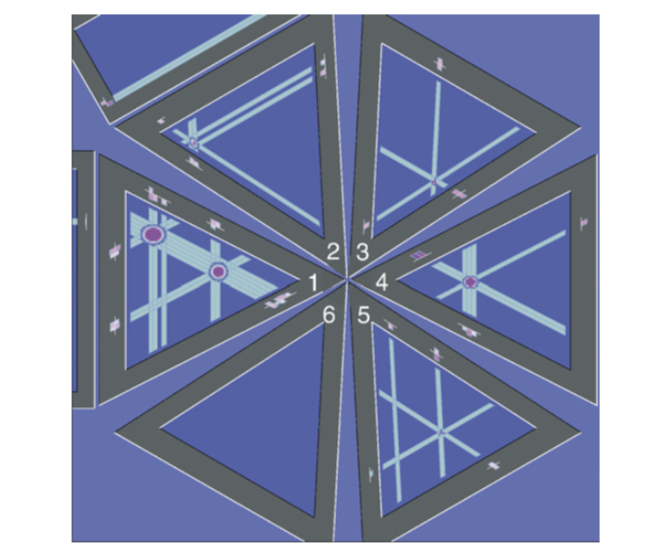
\includegraphics[]{figs/detectors/ec_sectors}
% \begin{figure}
% %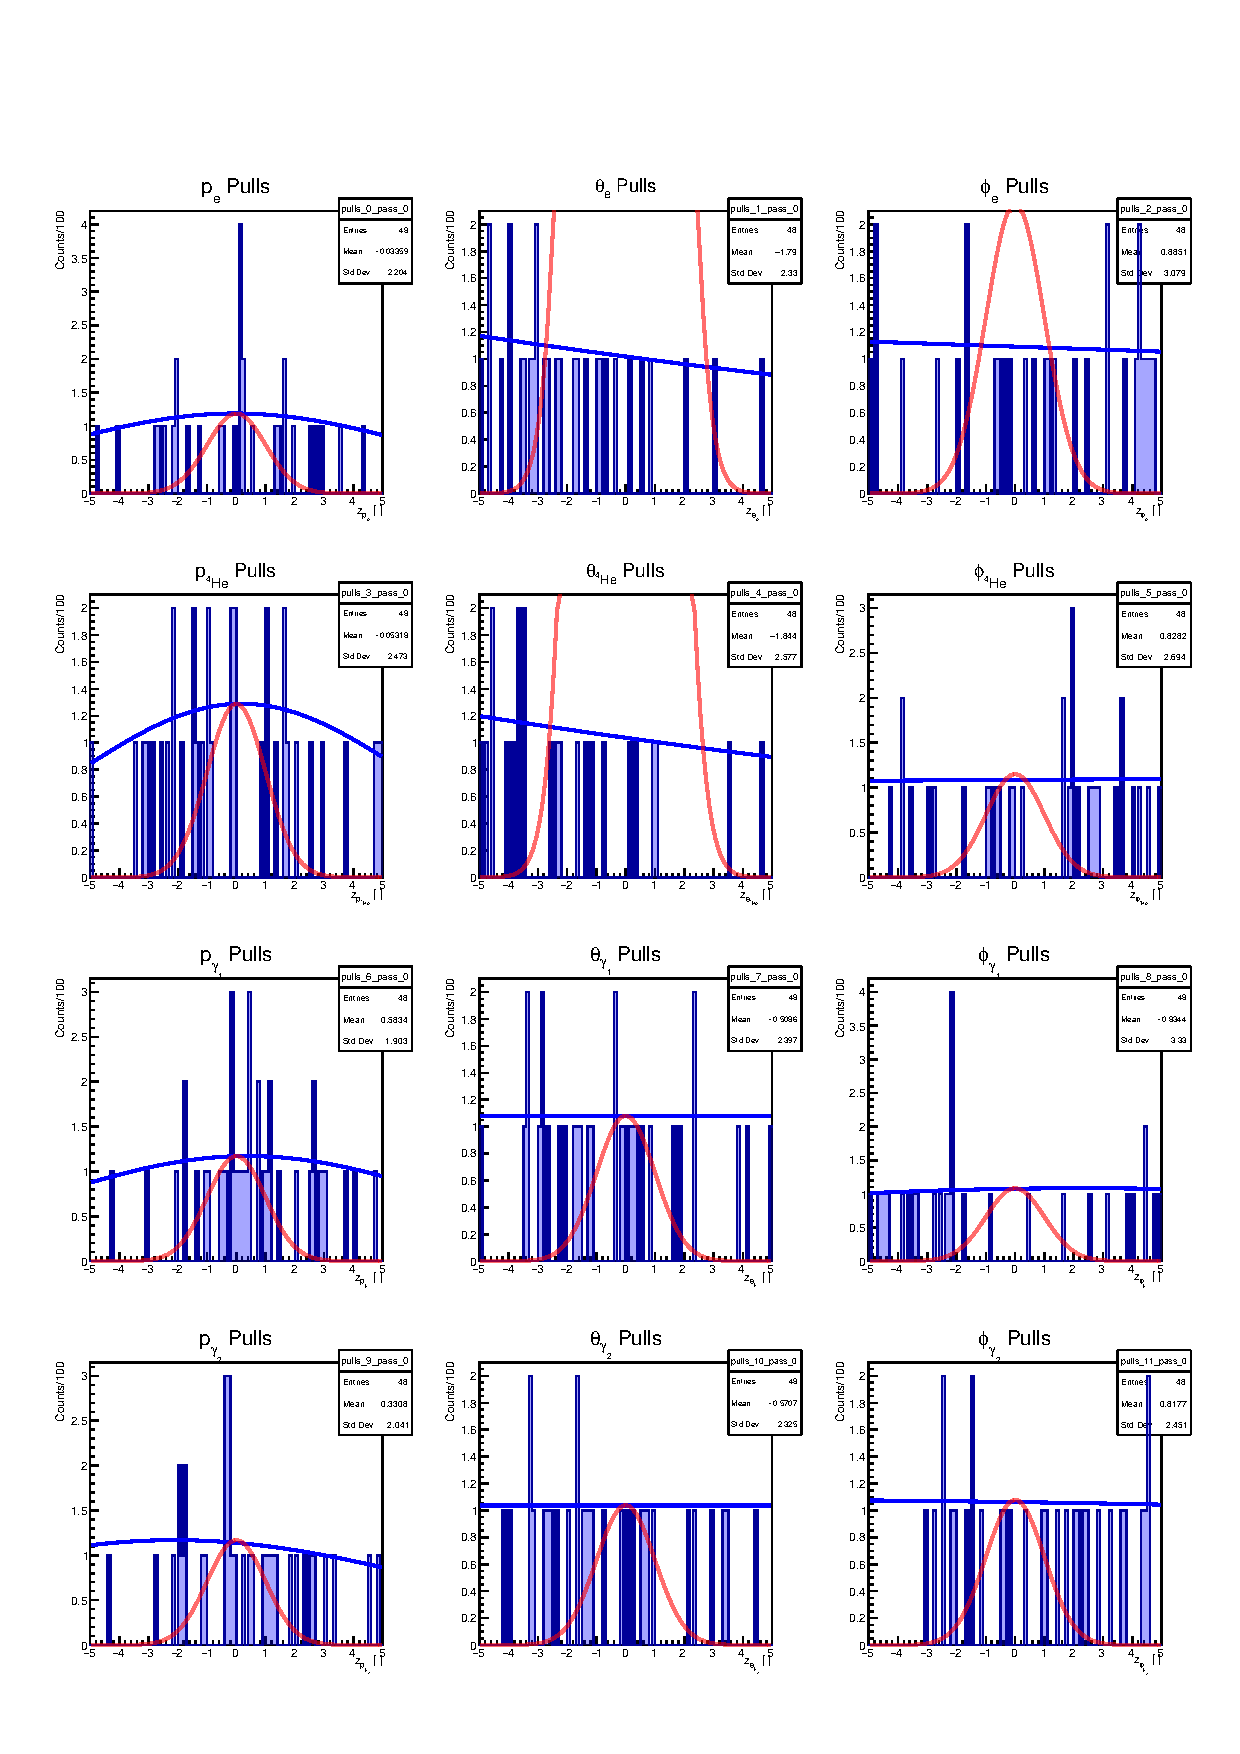
\includegraphics[width=\textwidth]{figs/dvcs/pulls}%
% 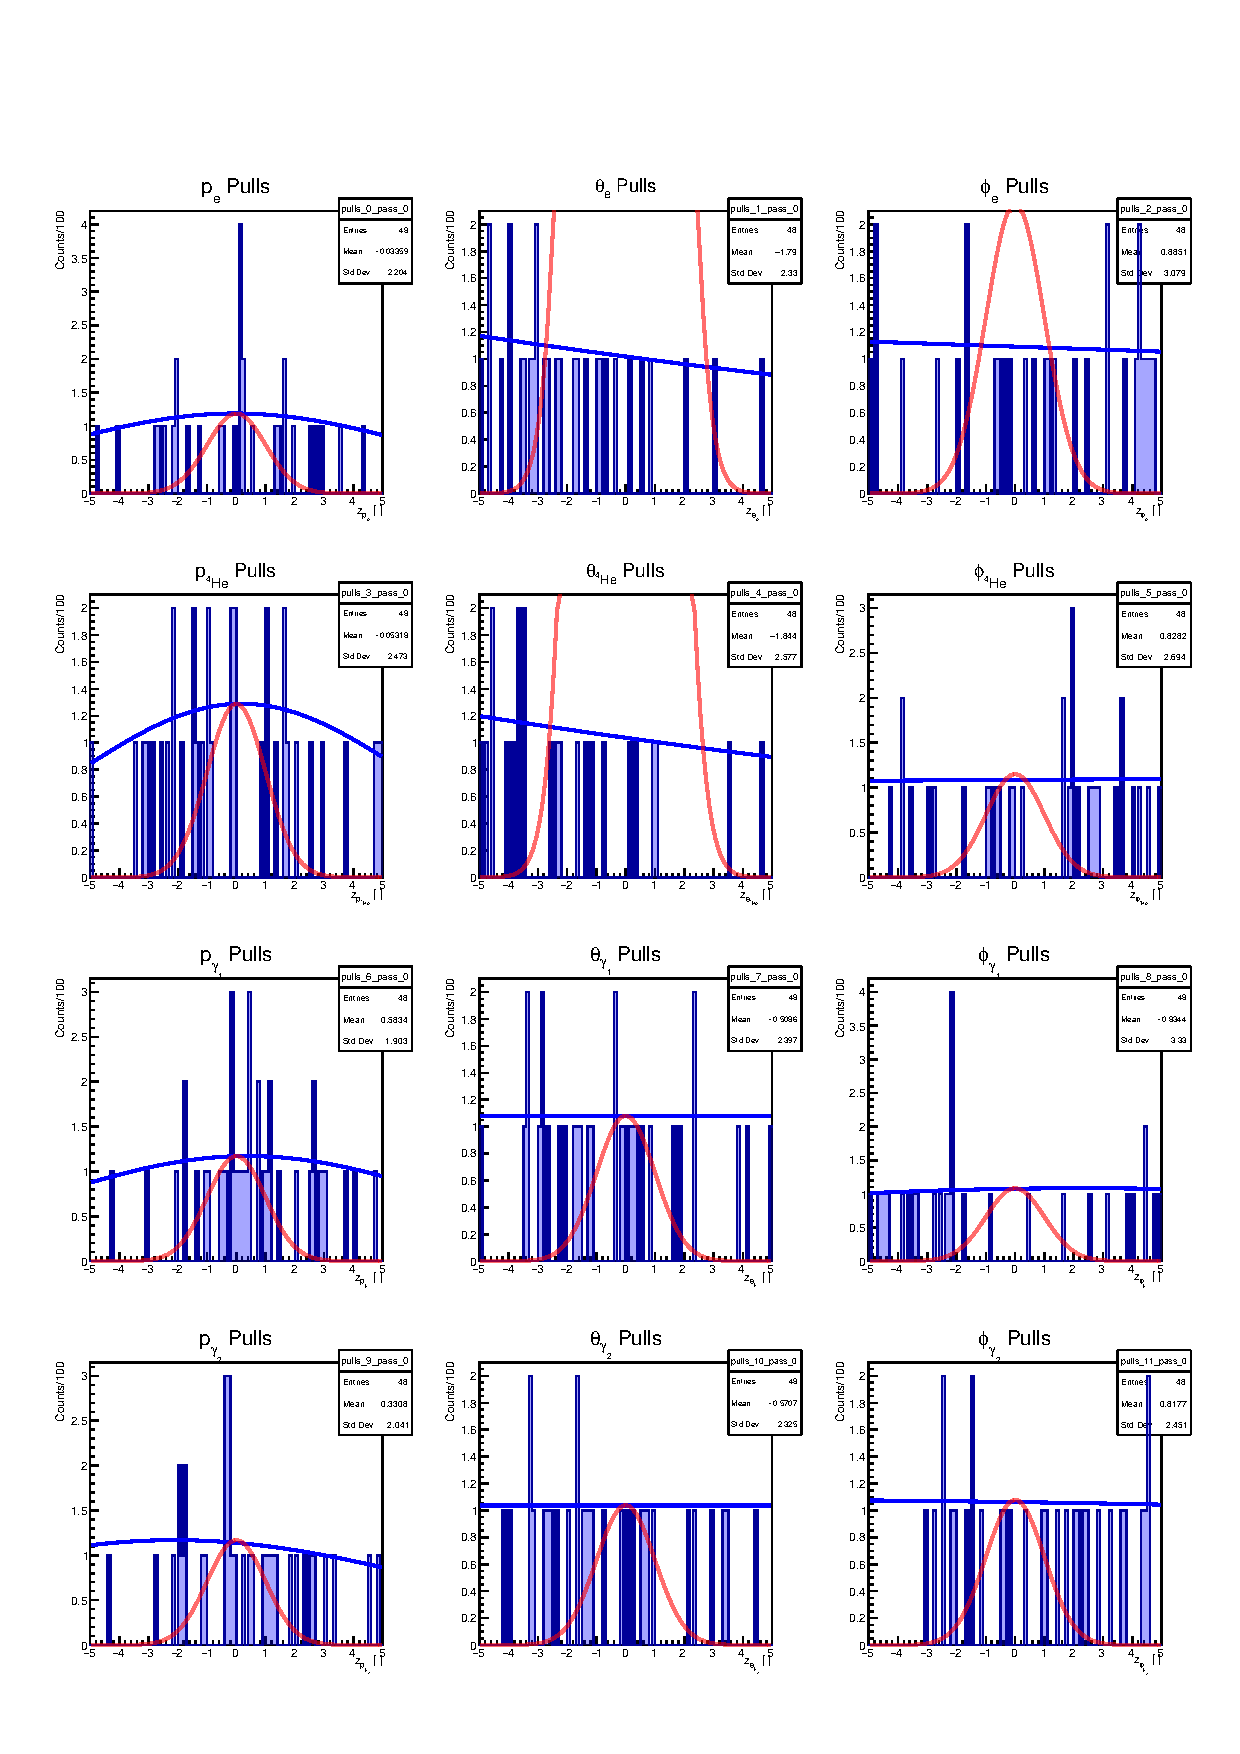
\includegraphics[width=50mm, scale=1]{figs/dvcs/pulls}%
% \caption{Caption of the fig\label{capp}}
% \end{figure}
%% Surround figure environment with turnpage environment for landscape
%% figure
% \begin{turnpage}
% \begin{figure}
%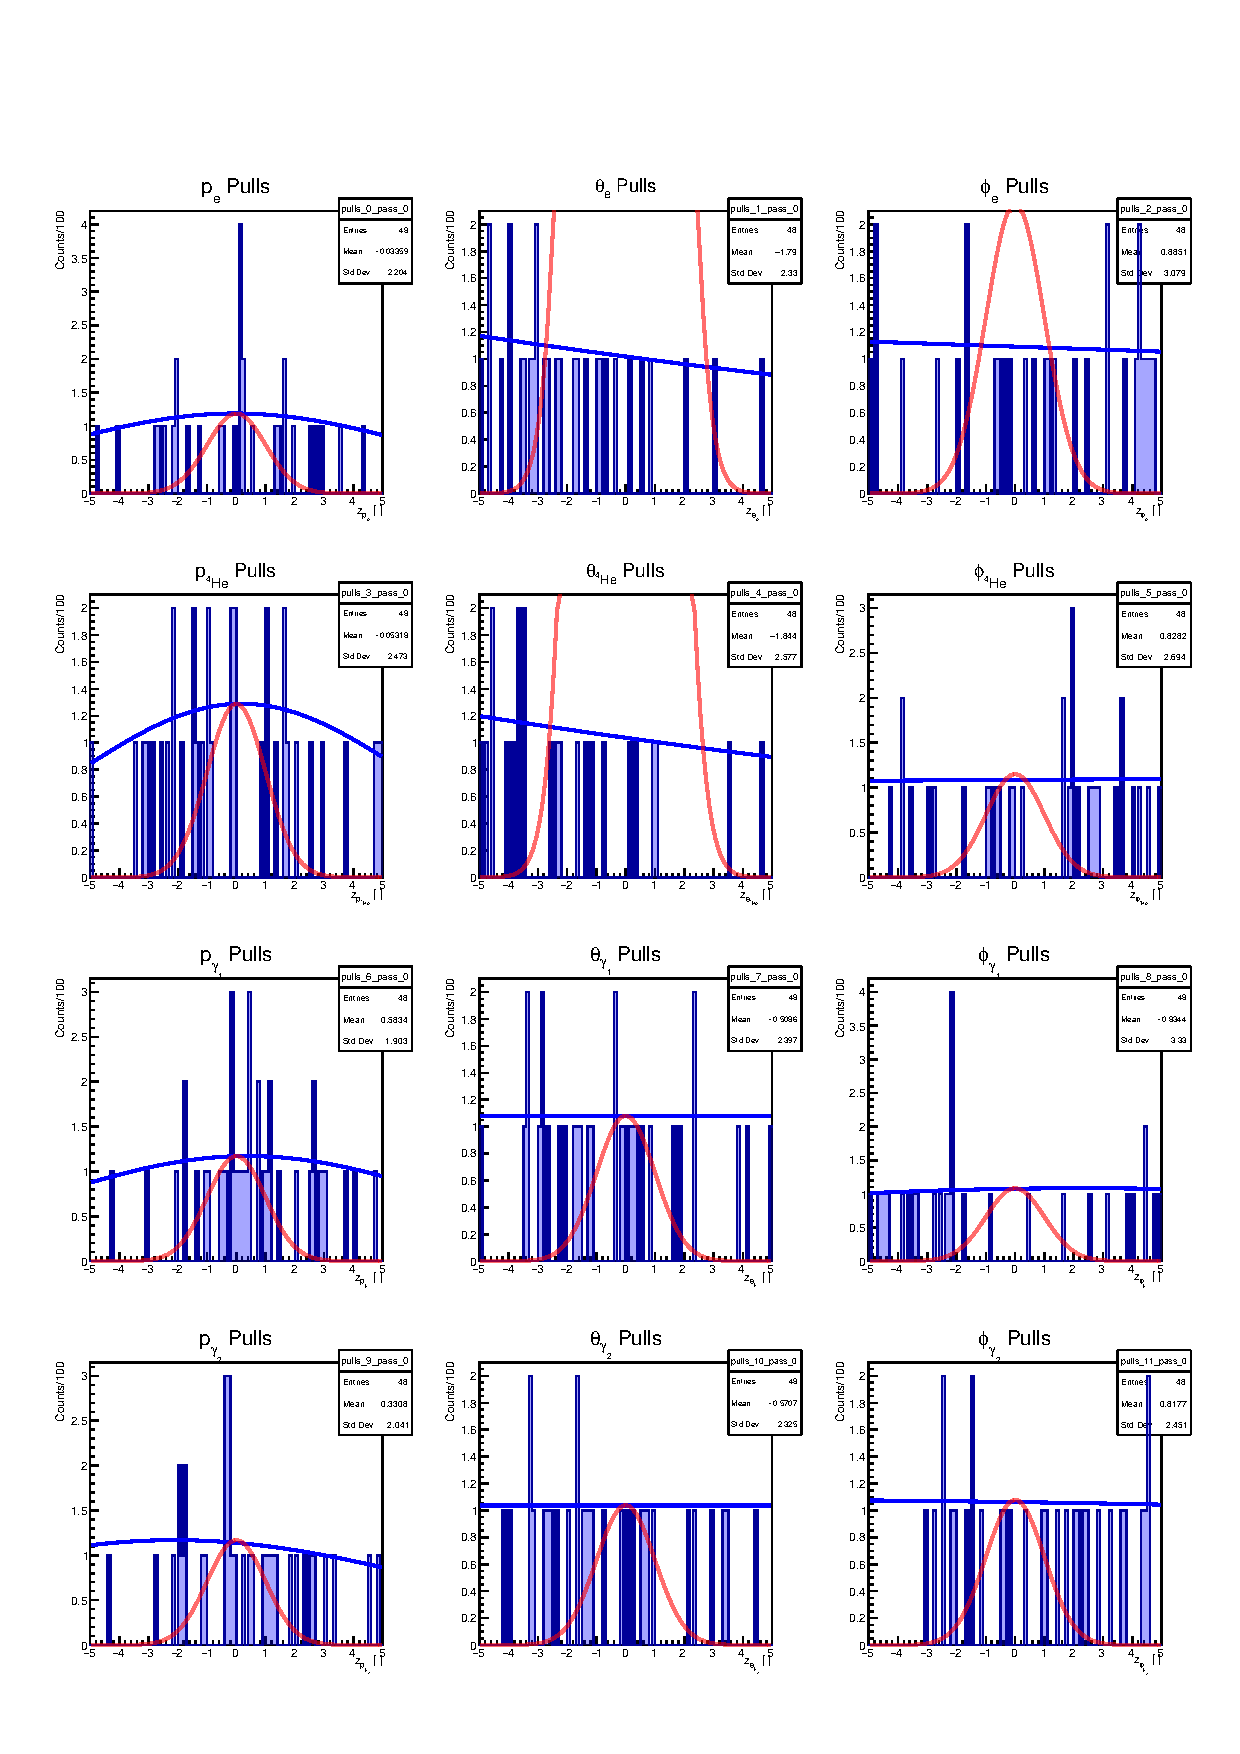
\includegraphics{figs/dvcs/pulls}%
% \caption{captionnnn \label{ test}}
% \end{figure}
% \end{turnpage}
% tables should appear as floats within the text
%
% Here is an example of the general form of a table:
% Fill in the caption in the braces of the \caption{} command. Put the label
% that you will use with \ref{} command in the braces of the \label{} command.
% Insert the column specifiers (l, r, c, d, etc.) in the empty braces of the
% \begin{tabular}{} command.
% The ruledtabular enviroment adds doubled rules to table and sets a
% reasonable default table settings.
% Use the table* environment to get a full-width table in two-column
% Add \usepackage{longtable} and the longtable (or longtable*}
% environment for nicely formatted long tables. Or use the the [H]
% placement option to break a long table (with less control than 
% in longtable).
% \begin{table}%[H] add [H] placement to break table across pages
% \caption{\label{}}
% \begin{ruledtabular}
% \begin{tabular}{}
% Lines of table here ending with \\
% \end{tabular}
% \end{ruledtabular}
% \end{table}

% Surround table environment with turnpage environment for landscape
% table
% \begin{turnpage}
% \begin{table}
% \caption{\label{}}
% \begin{ruledtabular}
% \begin{tabular}{}
% \end{tabular}
% \end{ruledtabular}
% \end{table}
% \end{turnpage}

% Specify following sections are appendices. Use \appendix* if there
% only one appendix.
%\appendix
%\section{}
% ****** End of file apstemplate.tex ******






\end{document}




%% Use math symbols (for bigoplus, etc)
%\usepackage{amssymb}
%% Formatting sections to have subsubsubsection
%\usepackage{titlesec} 
%    %\titlelabel{\thetitle.\quad}
%    %\titleformat{\section}{\normalfont\normalsize\bfseries}{\thesection}{5em}{}
%    \titlespacing*{\section}{0pt}{5ex plus 8ex minus 10ex}{5ex plus 5ex}
%    \titleclass{\subsubsubsection}{straight}[\subsection]
%    \newcounter{subsubsubsection}[subsubsection]
%    \renewcommand\thesubsubsubsection{\thesubsubsection.\arabic{subsubsubsection}}
%    \renewcommand\theparagraph{\thesubsubsubsection.\arabic{paragraph}} % optional; useful if paragraphs are to be numbered
%    \titleformat{\subsubsubsection} {\normalfont\normalsize\bfseries}{\thesubsubsubsection}{1em}{}
%    \titlespacing*{\subsubsubsection}
%    {0pt}{3.25ex plus 1ex minus .2ex}{1.5ex plus .2ex}
%    \makeatletter
%    \renewcommand\paragraph{\@startsection{paragraph}{5}{\z@}%
%      {3.25ex \@plus1ex \@minus.2ex}%
%      {-1em}%
%      {\normalfont\normalsize\bfseries}}
%    \renewcommand\subparagraph{\@startsection{subparagraph}{6}{\parindent}%
%      {3.25ex \@plus1ex \@minus .2ex}%
%      {-1em}%
%      {\normalfont\normalsize\bfseries}}
%    %\def\toclevel@part{0}
%    %\def\toclevel@section{1}
%    %\def\toclevel@subsection{2}
%    %\def\toclevel@subsubsection{3}
%    \def\toclevel@subsubsubsection{4}
%    \def\toclevel@paragraph{5}
%    \def\toclevel@paragraph{6}
%    %\def\l@part{{0}{7em}{4em}}
%    %\def\l@section{{1}{0em}{1em}}
%    %\def\l@subsection{\@dottedtocline{2}{1em}{2em}}
%    %\def\l@subsubsection{\@dottedtocline{3}{4em}{3em}}
%    \def\l@subsubsubsection{\@dottedtocline{4}{7em}{4em}}
%    \def\l@paragraph{\@dottedtocline{5}{10em}{5em}}
%    \def\l@subparagraph{\@dottedtocline{6}{14em}{6em}}
%    \makeatother
%    \setcounter{secnumdepth}{4}
%    \setcounter{tocdepth}{4}
%
%%Adjust space after part/section/subsection number/index
%\usepackage{tocloft}% http://ctan.org/pkg/tocloft:w
%\setlength{\cftsecindent}{3.125em}
%\setlength{\cftsubsecindent}{\cftsecindent + 1.5 em}
%\setlength{\cftsubsubsecindent}{\cftsubsecindent + 2.25em + 0.125em - 0.0625em}
%%\setlength{\cftpartnumwidth}{1.5 em}% Set length of number width in ToC for \subsection
%\setlength{\cftpartnumwidth}{7 ex}% Set length of number width in ToC for \subsection
%%\renewcommand{\cftpartaftersnum}{.}%
%
%% Indent the first paragraph
%\usepackage{indentfirst}
%% Edit title page
%\usepackage{titling} 
%% Cite with .bbl and .bib elements
%\usepackage{cite}
%% Add appendex
%\usepackage[toc,page]{appendix} 
%
%% Equation numbers are within section
%\numberwithin{equation}{subsubsection}
%% Figure numbers are within section
%\numberwithin{figure}{section}
%% Table numbers are within section
%\numberwithin{table}{section}
%% Omit `.0` in equation numbers for non-existent subsections.
%\renewcommand*{\theequation}{%
%  \ifnum\value{subsubsubsection}=0 %
%    \ifnum\value{subsubsection}=0 %
%      \ifnum\value{subsection}=0 %
%        \thesection
%      \else
%        \thesubsection
%      \fi
%    \else
%      \thesubsubsection
%    \fi
%  \else
%    \thesubsubsection
%  \fi
%  .\arabic{equation}%
%}
%
%\renewcommand{\thepart}{\Roman{part}.}
%%\renewcommand{\thepart}{Part \Roman{part}.}
%\renewcommand{\thesection}{\arabic{section}}
%\renewcommand{\thesubsection}{\thesection.\arabic{subsection}}
%\renewcommand{\thesubsubsection}{\thesubsection.\arabic{subsubsection}}
%
%\renewcommand{\thefigure}{\thesection.\arabic{figure}}
%\renewcommand{\thetable}{\thesection.\arabic{table}}
%%\renewcommand{\theequation}{\thesection\arabic{equation}}
%%\renewcommand{\thesubsection}{\thesection\arabic{subsection}}
%
%% Do this to do in-line figures
%\newlength\myheight
%\newlength\mydepth
%\settototalheight\myheight{Xygp}
%\settodepth\mydepth{Xygp}
%\setlength\fboxsep{0pt}
%\newcommand*\inlinegraphics[1]{%
%  \settototalheight\myheight{Xygp}%
%  \settodepth\mydepth{Xygp}%
%  \raisebox{-\mydepth}{\includegraphics[height=\myheight]{#1}}%
%}%\raisebox{-\mydepth}{\fbox{
\includegraphics[height=\myheight]{figs/pid/dots}}} hi 
%% Packages used in UMass Thesis
%%\usepackage{listings}
%%\usepackage{comment, cancel}
%
%% Set subtitle
%\newcommand{\subtitle}[1]{%
%  \posttitle{%
%    \par\end{center}
%    \begin{center}\large#1\end{center}
%    \vskip0.5em}%
%}
%\newcommand\pbwo{\ce{PbWO$_4$}}
%\newcommand\dimethyl{\ce{C$_2$H$_6$O}}
%\newcommand\CO{\ce{CO$_2$}}
%% Math Symbols
%%		\renewcommand{\lim}{\text{lim }}
%\renewcommand{\inf}{\text{inf }}
%\renewcommand{\max}{\text{max }}
%\renewcommand{\min}{\text{min }}
%\newcommand{\Res}{\text{Res }}				
%\newcommand\opcl[1]{\left [#1 \right)}
%\newcommand\diag[1]{\text{diag}\lr{#1}}
%\newcommand\I{{\mathbb I}}	
%\newcommand\bigO{\mathcal O}
%\newcommand{\vect}[1]{\vv{\bm{#1}}}
%\newcommand{\hatt}[1]{\hat{\bm{#1}}}
%\newcommand\fm{\phantom{-}}
%\newcommand\dd[2]{\frac{d #1}{d #2}}
%\renewcommand\d{\text{d}}
%\newcommand\bu[1]{\u{\b{#1}}}
%\newcommand\code[1]{\texttt{#1}}
%\newcommand\pct{0.5}
%\newcommand\cm{\text{cm}}
%\newcommand\degg{\text{deg}}
%\newcommand\corr{\text{corr}}
%\newcommand\meas{{\text{meas}}}
%
%% Header and Footer
%\renewcommand\hdsep{28pt}
%\hdrL{}
%\hdrC{Coherent DV$\pio$P with CLAS EG6} %HW Assignment Number
%\hdrR{} %Section and Assignment problems
%\ftrL { \\ November 2018 } %Subject and Professor
%\ftrC {Exclusive $\pio$ Electroproduction Off $\he$}
%\ftrR { \PgNo}%Assignment problems continued
%
%
%
%
%\usepackage{amsmath}
%% Has lVert and rVert for absolute value and norm environments
%\usepackage{mathtools}
%\DeclareMathSymbol{.}{\mathpunct}{letters}{"3A}
%\DeclareMathSymbol{,}{\mathpunct}{letters}{"3B}	
%\DeclarePairedDelimiter\ceil{\lceil}{\rceil}
%\DeclarePairedDelimiter\floor{\lfloor}{\rfloor}
%\DeclarePairedDelimiter\norm{\lVert}{\rVert}%
%
%% Horizontal dashed lines
%\usepackage{dashrule}
%\renewcommand\newline{ \vspace{\baselineskip}}
%\newcommand\hdash[1]{ \noindent\hfill\hdashrule[0.5ex]{#1\textwidth}{0.5pt}{1mm}\hfill \newline }
%\newcommand\hLine[1]{ \noindent\hfill\rule{#1\textwidth}{.4pt}\hfill \newline }
%  
%\newcommand\EC{\text{EC}}
%\newcommand\IC{\text{IC}}
%\newcommand\DC{\text{DC}}
%\newcommand\RTPC{\text{RTPC}}
%
%% Use captions and subcaptions for figures and subfigures
%\usepackage[font=footnotesize,labelfont={bf},tableposition=top]{caption}
%\usepackage[font=scriptsize,labelfont={bf}]{subcaption}
%%% Have figure next to table
%%\usepackage{floatrow}
%%    \usepackage{blindtext}
%%    % Table float box with bottom caption, box width adjusted to content
%%    \newfloatcommand{capbtabbox}{table}[][\FBwidth]
%%    \renewfloatcommand{ffigbox}{figure}[][\FBwidth]
%%\usepackage[]{tocbibind}
%
%% Add bib to table of contents
%% Use for appendix numbers and counters
%\usepackage{etoolbox}
%%\apptocmd{\thebibliography}{\csname phantomsection\endcsname\addcontentsline{toc}{chapter}{References}}{}{}
%%    \setcounter{tocdepth}{4}
%%    \setcounter{secnumdepth}{4}
%
%% Referencing a list of references
%\usepackage{cleveref}
%
%
%% help with appendix issues
%\newenvironment{boldenv}{\bfseries} % I use this if adding text to a plot, then screen shot and gimp it
%
%\AtBeginEnvironment{thebibliography}{\linespread{1}\selectfont} % this single spaces the bib which was driving me nuts
%
%\begin{document}
